\documentclass[11pt, a4paper, oneside]{report} 
\setcounter{secnumdepth}{3} % Numbers subsubsections (1.1.1)
\setcounter{tocdepth}{2}    % Shows down to subsections in TOC

% --- Packages ---
\usepackage[utf8]{inputenc}
\usepackage[T1]{fontenc}
\usepackage{geometry}
\geometry{
    a4paper,
    margin=2.5cm, % Equal 2.5cm margins everywhere (standard for drafts)
    % bindingoffset=0cm % Use this if you print later
}
\usepackage{graphicx} % Remove [demo] when you have real images
\usepackage{amsmath, amssymb, amsthm}
\usepackage{setspace}
\usepackage[linesnumbered,ruled,vlined]{algorithm2e}
\usepackage{subcaption}
\usepackage[font=small, labelfont=bf]{caption} % Nicer captions
\usepackage{microtype} % The "secret weapon" for pro typography
\usepackage{tikz}

\usetikzlibrary{
    decorations.pathmorphing, % Required for "random steps" (The schematic)
    positioning,              % Required for "right=of" (The new diagrams)
    arrows.meta,              % Required for ">=Latex" arrowheads
    shapes,                   % Required for node shapes
    calc,                     % Required for coordinate calculations
    backgrounds,               % Optional but good for complex figures
    angles,
    quotes,
    decorations.markings
}

% --- Bibliography & Links ---
\usepackage[numbers, sort&compress]{natbib} % Numbered citations [1-3]
\usepackage[colorlinks=true, linkcolor=blue, citecolor=blue, urlcolor=blue]{hyperref} % Blue links, no boxes
\usepackage{cleveref} % Smart referencing (load after hyperref)
\usepackage{fancyhdr}

% --- Aesthetic Setup ---
\setlength{\parskip}{0em} % Small space between paragraphs
\setstretch{1.2} % Requires \usepackage{setspace}

% Header/Footer Style
\pagestyle{fancy}
\fancyhf{}
\fancyhead[LE,RO]{\thepage} % Page number on outer corners
\fancyhead[RE]{\leftmark}   % Chapter title on inner (even pages)
\fancyhead[LO]{\rightmark}  % Section title on inner (odd pages)
\renewcommand{\headrulewidth}{0.4pt}

% Theorem Environments
\newtheorem{theorem}{Theorem}[chapter]
\newtheorem{definition}{Definition}[chapter]
\newtheorem{lemma}{Lemma}[chapter]
\newtheorem{proposition}{Proposition}[chapter]
\newtheorem{remark}{Remark}[chapter]
\newtheorem{corollary}{Corollary}[chapter]

\begin{document}


% --- Title Page ---
\begin{titlepage}
    \centering
    \vspace*{2cm}
    
    {\Huge \bfseries Diffusion Limited Aggregation \par}
    
    \vspace{2cm}
    
    {\Large \textbf{Candidate Number: [Your Number]} \par}
    \vspace{1cm}
    {\large Hilary Term 2026 \par}
    
    \vspace{4cm}
    
    \includegraphics[width=0.3\textwidth]{example-image-a} % Replace with University Logo
    
    \vspace{3cm}
    
    {\large \itshape A dissertation submitted for the degree of\\
    Mathematics Part B \par}
    
\end{titlepage}

% --- Abstract ---
\thispagestyle{plain}
\begin{center}
    {\Large \bfseries Abstract}
\end{center}
\vspace{0.5cm}
\begin{quote}
    This dissertation investigates the universality class of Diffusion Limited Aggregation (DLA) through the lens of conformal mapping and harmonic measure theory. We compare on-lattice, off-lattice, and hybrid "snapping" algorithms to determine if microscopic lattice anisotropy survives in the macroscopic scaling limit. Particular attention is paid to the dimension of the harmonic measure and the dynamics of the active growth zone. [Placeholder: Finish this summary with your specific results regarding the Hybrid model's classification, totaling approx. 300 words.]
\end{quote}
\newpage

% --- TOC ---
\tableofcontents
\newpage

% --- Main Content ---
% =========================================
% CHAPTER 1: INTRODUCTION
% =========================================
\chapter{Introduction}
\label{ch:intro}

\section{Overview}
Diffusion Limited Aggregation (DLA) is a stochastic model for irreversible colloidal aggregation. In this model a seed particle is placed at the origin, and then subsequent particles are released from a boundary far from the cluster one at a time. The particle then diffuses, either as a random walk on a lattice or Brownian motion (the continuous analogue to a random walk). Upon collision, the walker sticks and the next one starts diffusing.

The model was first proposed in 1981 by Witten and Sander to model the colloidal aggregation of metal precipitates \cite{witten1981}, but has since been found to have applications in a diverse range of physical systems, including electrodeposition \cite{Matsushita1984}, bacteria growth \cite{BenJacob1994} and viscous fingering in Hele-Shaw cells \cite{Paterson1984} among others.

%first visual of DLA
% --- FIGURE 1.2: REAL VS SIMULATION ---
\begin{figure}[ht]
    \centering
    % --- Panel A: Nature (Zinc) ---
    \begin{subfigure}[b]{0.3\textwidth}
        \centering
        % You need to screenshot this from Matsushita (1984) and save as zinc.png
        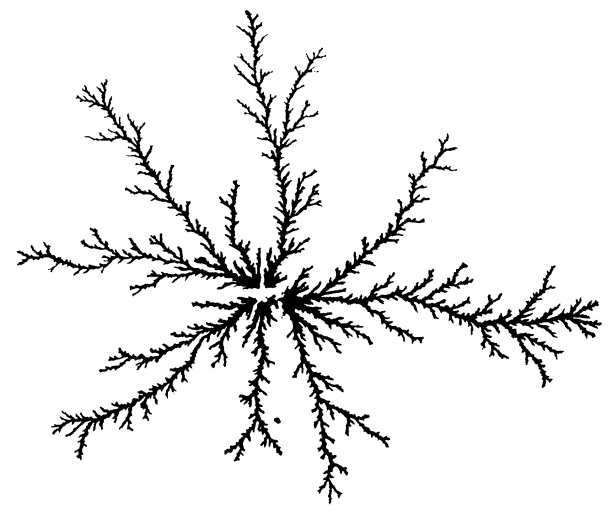
\includegraphics[width=\textwidth, trim=0 0 0 1.5cm, clip]{images/zinc_intro.png} 
        \caption{Zinc Electrodeposition \cite{Matsushita1984}}
        \label{fig:zinc}
    \end{subfigure}
    \hfill % Adds flexible space
    % --- Panel B: Off-Lattice ---
    \begin{subfigure}[b]{0.3\textwidth}
        \centering
        % Note: 'trim' cuts off the header. Adjust '1.5cm' if needed.
        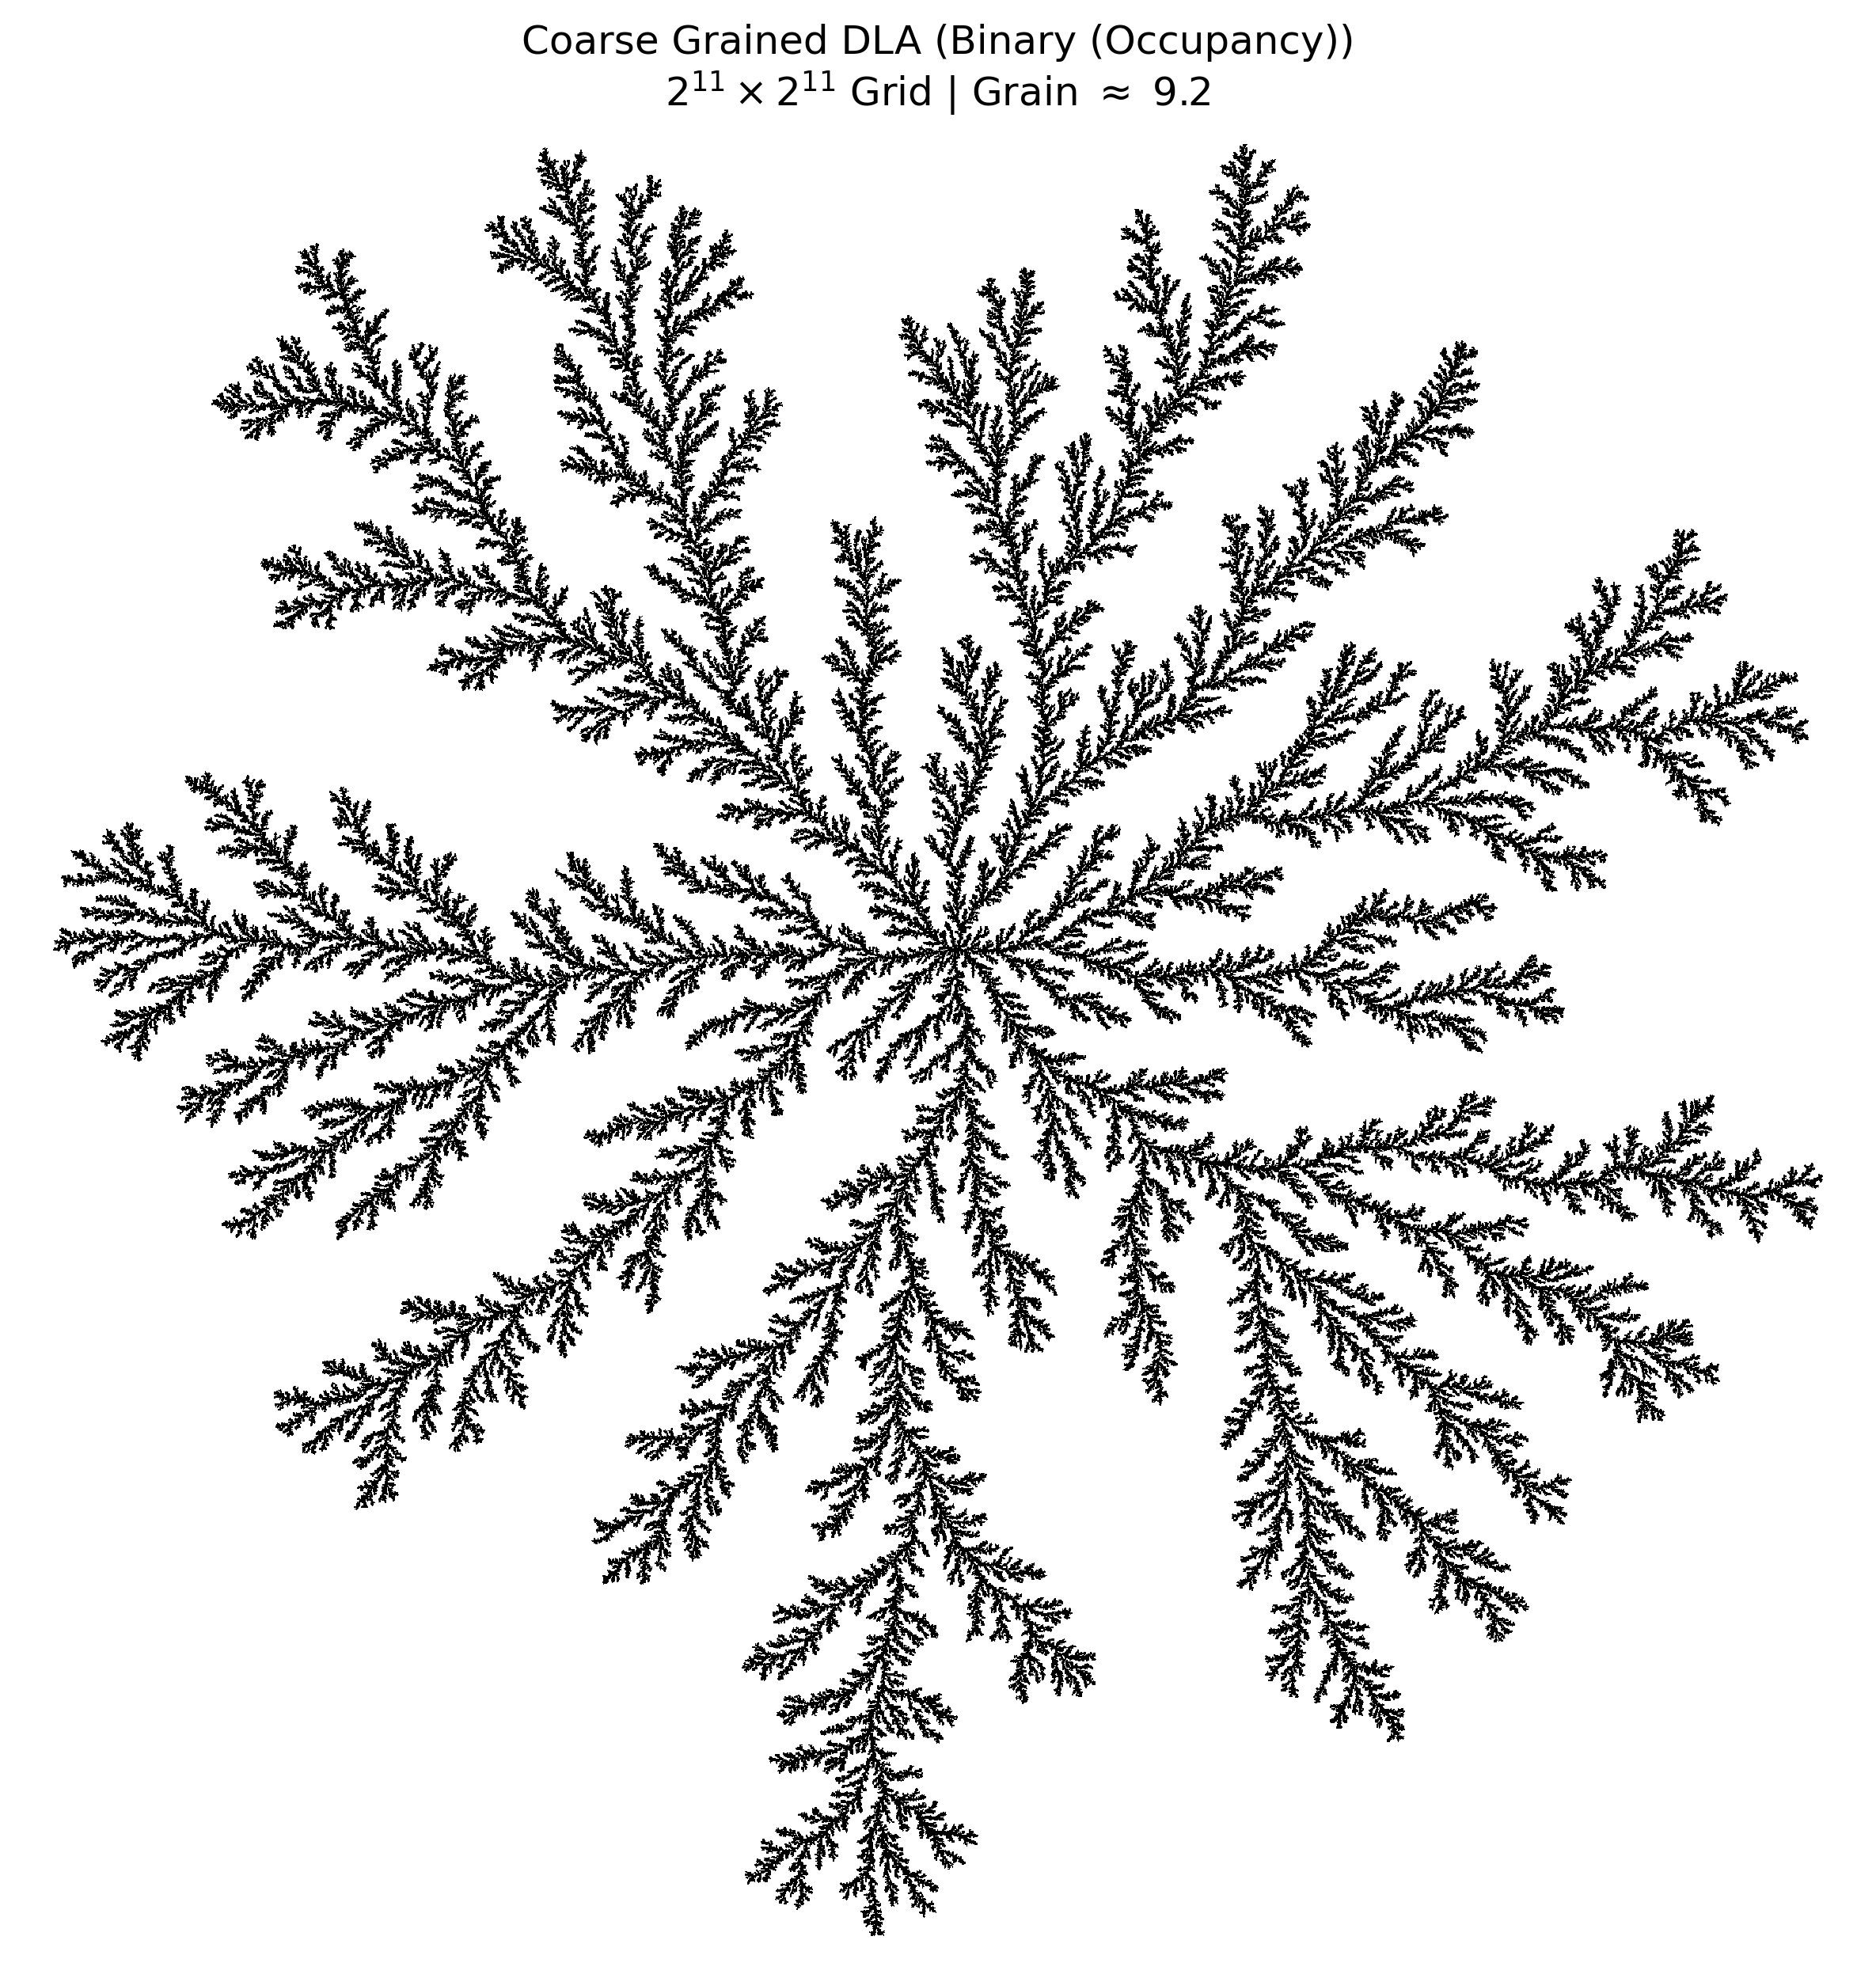
\includegraphics[width=\textwidth, trim=0 0 0 1.5cm, clip]{images/off_lattice_intro.png} 
        \caption{Off-Lattice DLA}
        \label{fig:off_lattice_intro}
    \end{subfigure}
    \hfill
    % --- Panel C: On-Lattice ---
    \begin{subfigure}[b]{0.3\textwidth}
        \centering
        % Note: 'trim' cuts off the header.
        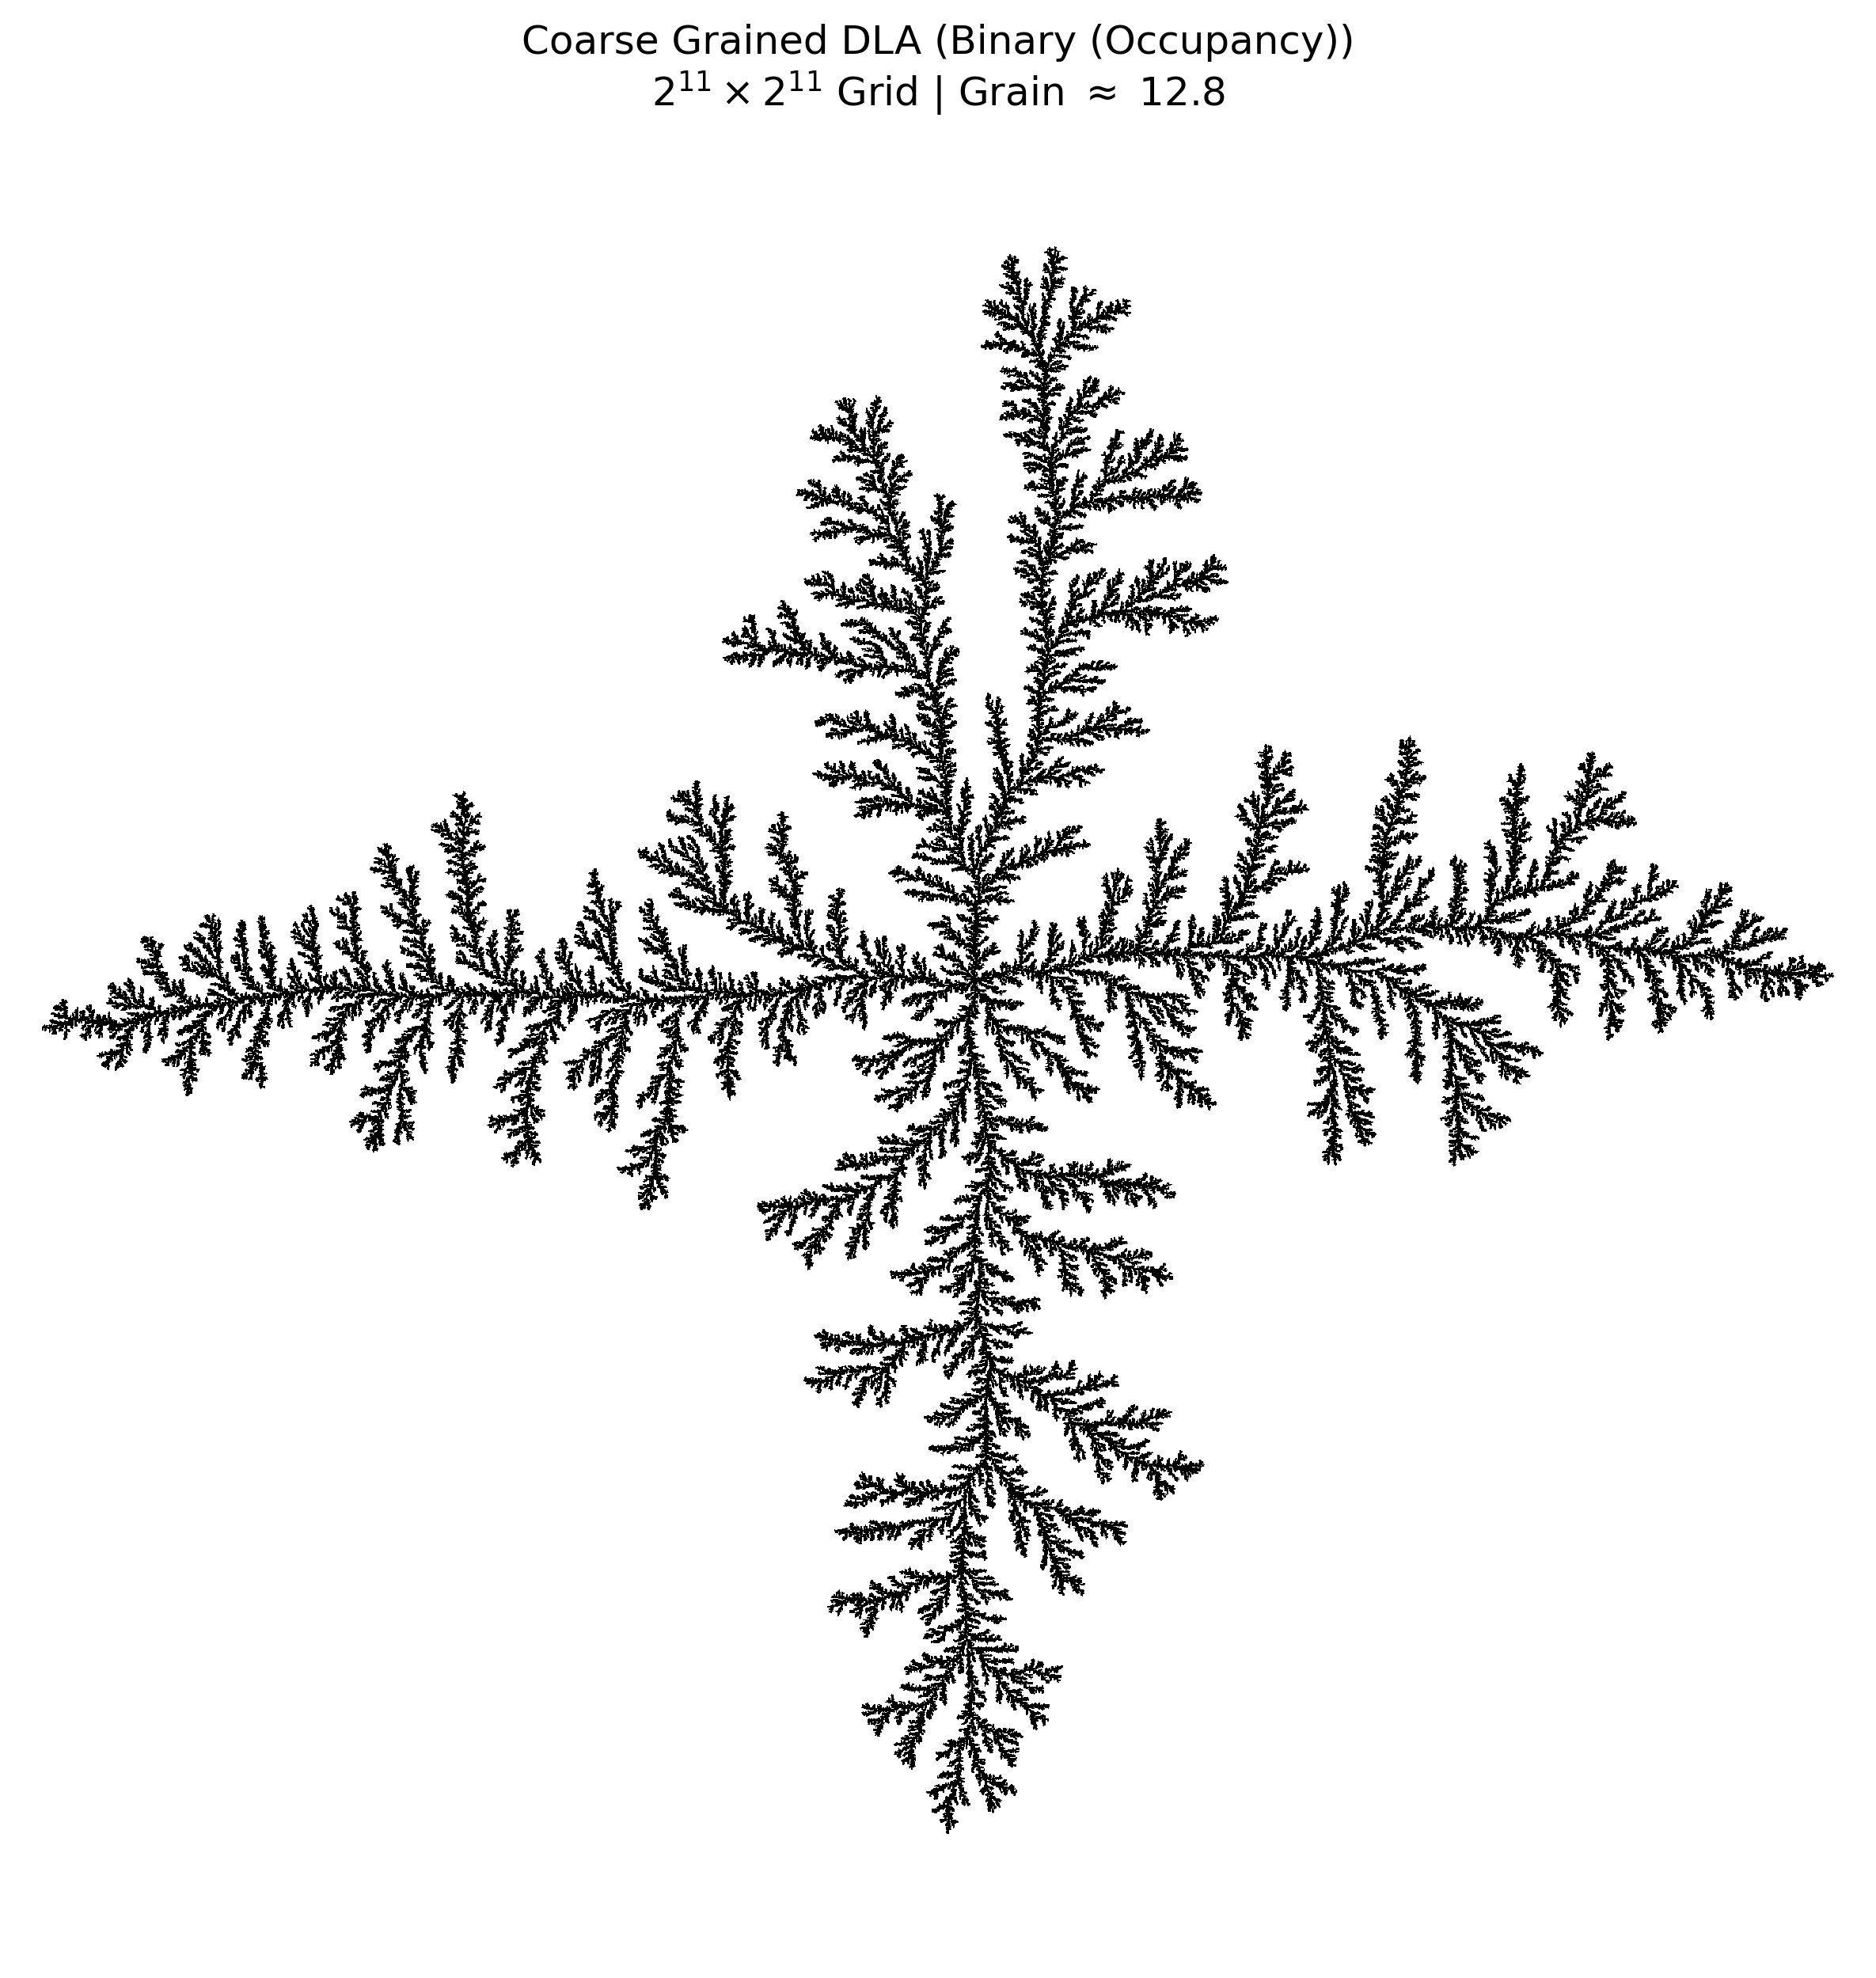
\includegraphics[width=\textwidth, trim=0 0 0 1.5cm, clip]{images/on_lattice_intro.png} 
        \caption{On-Lattice DLA}
        \label{fig:on_lattice_intro}
    \end{subfigure}
    
    \caption{Comparison of physical aggregation (a) with the two primary modelling approaches: continuum Off-Lattice DLA (b) and discrete On-Lattice DLA (c). Both are the results of simulation with $10^7$ particles. Note the distinct grid-induced anisotropy visible in the on-lattice case.}
    \label{fig:three_panel_comparison}
\end{figure}

\section{Theoretical Context}
While DLA is defined by a stochastic algorithm (random walkers), its theoretical significance lies in its connection to potential theory, the study of harmonic functions. As will be detailed in the following chapters, the probability density $\phi(u)$ of a diffusing particle at position $u$ satisfies the Laplace equation $\nabla^2 \phi = 0$. Intuitively, this is because both random walks and harmonic functions are defined by the property that the value at any point is the average of its neighbours. Each additional walker to aggregate onto the cluster distorts this probability field, creating a Laplacian instability that amplifies irregularities into the observed complicated structure \cite{Lawler2010}.

\section{Fractal Dimension}
Visually, DLA clusters exhibit self-similarity, where small branches look statistically identical to large branches. Mathematically this can be understood via fractal dimension $D$. This will be formally defined later, but can be thought of as the relationship between the mass of a cluster (number of particles $N$) and its linear size $R$, where:
\begin{equation}
    N \propto R^D.
\end{equation}
For instance, doubling the size of a line would double its mass, so it has dimension 1, while doubling the size of a solid disc would quadruple its mass, so this has dimension 2. Simulations of off-lattice DLA have consistently yielded a fractal dimension $D \approx 1.71$, but this has not been proven \cite{Meakin1983}.

In fact, the only mathematical theorem on 2D DLA is due to Kesten, who proved a bound on the growth rate of on-lattice DLA in 1987, with a key consequence being that the fractal dimension of a DLA cluster is bounded below by $1.5$ \cite{Kesten1987}.

\section{Anisotropy and Thesis Goals}
It is likely that the dimension of on-lattice DLA is actually lower than off-lattice due to the effect of the grid on the cluster shape, a phenomenon known as anisotropy. Grebenkov and Beliaev discussed how anisotropy is likely to reduce the dimension of large enough clusters \cite{Grebenkov2017}, but understanding why and to what extent is still not fully understood.

To answer these questions, simulations of DLA must be done both on and off-lattice. Additionally, to understand the effect of the lattice we create a 'hybrid' algorithm with continuous diffusion but a discrete aggregation method. Other hybrid models of DLA have previously been studied \cite{Shmyrov2019}, including a similar semi-lattice approach \cite{Menshutin2011}, but to our knowledge have not been utilised to decouple the effects of transport from aggregation in on-lattice DLA.

The purpose of this dissertation is to compare these three different models of DLA, in order to decouple the diffusion process of DLA from the geometry of the aggregation. By analysing various features of the resulting clusters, we hope to better understand the relationship between the continuous and discrete variations of the probability distribution governing DLA growth.

We begin with a brief outline of the mathematical necessary to understand the underlying mechanisms behind DLA in \cref{ch:theory}, before following on by explaining how to utilise this theory to create efficient algorithms, as well as discussing our hybrid approach, which forms \cref{ch:algorithms}. In ?? we begin analysis, focusing on ??? 
% =========================================
% CHAPTER 2: POTENTIAL THEORY
% =========================================
\chapter{Potential Theory}
\label{ch:theory}

\section{Preliminaries} % may end up in appendix
\label{sec:preliminaries}

\subsection{Martingales and the Optional Stopping Theorem}
In this section, we review the probabilistic tools required to link random walks to potential theory. We assume standard measure-theoretic knowledge (equivalent to the Part A Integration course).

\begin{definition}[Probability Space]
A probability space $(\Omega, \mathcal{F}, \mathbb{P})$ is a triple where $\Omega$ is a sample set, $\mathcal{F}$ is a $\sigma$-algebra on $\Omega$ representing the set of events, and $\mathbb{P} \colon \mathcal{F}\to[0,1]$ is a countably additive set function such that $\mathbb{P}(\Omega)=1$.
\end{definition}

\begin{definition}[Filtration]
A filtration on a probability space $(\Omega, \mathcal{F}, \mathbb{P})$ is a sequence of sub-$\sigma$-algebras $(\mathcal{F}_n)_{n \geq 0}$ such that:
\begin{equation*}
    \mathcal{F}_0 \subseteq \mathcal{F}_1 \subseteq \mathcal{F}_2 \subseteq \dots \subseteq \mathcal{F}.
\end{equation*}
The tuple $(\Omega, \mathcal{F}, (\mathcal{F}_n)_{n \geq 0}, \mathbb{P})$ is called a filtered probability space.
\end{definition}

\noindent \textit{Intuition:} The filtration $(\mathcal{F}_n)$ represents the accumulation of information over time. $\mathcal{F}_n$ contains all events whose occurrence (or non-occurrence) is known by time $n$.

\begin{definition}[Stopping Time]
A random variable $\tau \colon \Omega \to \{0, 1, \dots, \infty\}$ is called a stopping time with respect to the filtration $(\mathcal{F}_n)_{n \geq 0}$ if for every $n \geq 0$:
\begin{equation*}
    \{ \omega \in \Omega : \tau(\omega) \leq n \} \in \mathcal{F}_n.
\end{equation*}
\end{definition}

\noindent \textit{Intuition:} A stopping time represents a strategy where the decision to stop at time $n$ depends only on the history of the process up to time $n$. For example, ``stop when the walker hits the cluster" is a valid stopping time but ``stop at the step before the walker hits the cluster" is not.

\begin{definition}[Martingale]
A discrete-time stochastic process $(X_n)_{n \geq 0}$ is a martingale with respect to a filtration $(\mathcal{F}_n)_{n \geq 0}$ if:
\begin{enumerate}
    \item $X_n$ is adapted to the filtration (i.e., $X_n$ is $\mathcal{F}_n$-measurable for all $n$),
    \item $\mathbb{E}[|X_n|] < \infty$ for all $n$ (integrability),
    \item $\mathbb{E}[X_{n+1} \mid \mathcal{F}_n] = X_n$ almost surely (conditional expectation).
\end{enumerate}
\end{definition}

\noindent \textit{Intuition:} A martingale models a ``fair game" with no drift. The condition $\mathbb{E}[X_{n+1} \mid \mathcal{F}_n] = X_n$ implies that given the entire history of the process, the best prediction for the next value is the current value.

\begin{theorem}[Doob's Optional Stopping Theorem]
\label{thm:ost}
    Let $X$ be a martingale on a filtered probability space. If $\tau$ is a stopping time such that $\mathbb{P}(\tau < \infty) = 1$, and $X$ is uniformly bounded (i.e., there exists $K$ such that $|X_n(\omega)| \leq K$ for all $n, \omega$), then:
\begin{equation}
    \mathbb{E}[X_\tau] = \mathbb{E}[X_0].
\end{equation}
\end{theorem}

\begin{proof}
See \citet[Section 10.9]{Williams1991}.
\end{proof}

\noindent \textit{Intuition:} The Optional Stopping Theorem states that for a fair game, no stopping strategy $\tau$ can change the expected payout. This will allow us to relate the value of a harmonic function at a starting point $x$ (start of the walk) to its expected value at the boundary $\partial D$ (end of the walk).

\subsection{Measure Theory Concepts}

In the study of potential theory, we will want to understand the relationship between the geometric length of a boundary (Lebesgue measure) and the probability that a random walker hits that boundary (harmonic measure). To rigorously define a probability density function linking these two concepts we require the notion of the Radon-Nikodym derivative.

\noindent \textit{Remark:} throughout this work, we assume our measurable spaces are equipped with the Borel $\sigma$-algebra.
\begin{definition}[Absolute Continuity]
Let $(\Omega, \mathcal{F})$ be a measurable space equipped with two measures $\mu$ and $\nu$. We say that $\nu$ is absolutely continuous with respect to $\mu$, denoted $\nu \ll \mu$, if for every $A \in \mathcal{F}$:
\begin{equation}
    \mu(A) = 0 \implies \nu(A) = 0.
\end{equation}
\end{definition}

\noindent \textit{Intuition:} If $\nu \ll \mu$, then $\nu$ assigns zero mass to any set where $\mu$ assigns zero mass. This ensures that we can't have a "probability" of being in a region with zero "volume."

\begin{theorem}[The Radon-Nikodym Theorem]
Let $(\Omega, \mathcal{F})$ be a measurable space, and let $\mu$ and $\nu$ be two finite measures such that $\nu \ll \mu$. Then, there exists a non-negative measurable function $f \colon \Omega \to [0, \infty)$, unique $\mu$-almost everywhere, such that for any $A \in \mathcal{F}$:
\begin{equation}
    \nu(A) = \int_A f \, d\mu.
\end{equation}
The function $f$ is called the Radon-Nikodym derivative of $\nu$ with respect to $\mu$ and is denoted by:
\begin{equation}
    f = \frac{d\nu}{d\mu}.
\end{equation}
\end{theorem}

\begin{proof}
See \citet[Section 5.14]{Williams1991}.
\end{proof}

%add LCLT and also Ito's Lemma?

\subsection{Conformal Maps}

Here we state the definition of a conformal map, and the Riemann mapping theorem. Conformal maps will be very important for two reasons: theoretically, the Riemann Mapping Theorem guarantees that the Dirichlet problem is well-posed even on the fractal boundary of a DLA cluster; algorithmically, these maps allow us to exploit the 'conformal invariance' of Brownian motion (discussed later)
\begin{definition}[Conformal Map]
Let $U, V \subseteq \mathbb{C}$ be open sets. A function $f \colon U \to V$ is called \textbf{conformal} at a point $z_0 \in U$ if it preserves angles and orientation locally. 

Analytically, a holomorphic function $f$ is conformal at every point where its derivative is non-zero, i.e., $f'(z) \neq 0$. If $f$ is a holomorphic bijection between $U$ and $V$ (a biholomorphism), it is essentially a global conformal map, and we say $U$ and $V$ are conformally equivalent.
\end{definition}

\begin{theorem}[Riemann Mapping Theorem]
Let $U \subsetneq \mathbb{C}$ be a non-empty, simply connected open subset of the complex plane (i.e., $U$ is the whole plane minus at least one point, with no holes). Then, there exists a unique bijective conformal map $f$ from $U$ onto the open unit disk $\mathbb{D} = \{z \in \mathbb{C} : |z| < 1\}$ such that:
\begin{equation}
    f(z_0) = 0 \quad \text{and} \quad f'(z_0) > 0,
\end{equation}
for any prescribed point $z_0 \in U$.
\end{theorem}

\begin{proof}
See \citet[Chapter 6]{Ahlfors1979} or \citet[Chapter 9]{Priestley2003}.
\end{proof}

\section[Discrete Potential Theory]{Discrete Potential Theory\footnote{The theoretical framework in this section is largely adapted from \citet{Lawler2010}, applied here to the specific case of 2D DLA.}}\label{sec:discrete_theory}
We now introduce potential theory in a discrete setting, focusing on its applications to DLA. We start by considering the definitions of a random walk and a discrete harmonic function.
%remark about focusing on intuition and links to DLA, and therefore omitting proofs, which can be found in Lawler and Limic.
\subsection{Simple Random Walks and the Generator}
\label{sec:rw_generator}
\begin{definition}[Random Walk]
A random walk on $\mathbb{Z}^2$ is a stochastic process $(S_n)_{n \geq 0}$ defined by $S_n = S_0 + \sum_{i=1}^n X_i$, where $X_1, X_2, \dots$ are independent and identically distributed random variables taking values in $\mathbb{Z}^2$. 

The common distribution of the steps is denoted by $p(x) = \mathbb{P}(X_i = x)$ and is called the \textbf{increment distribution}.
\end{definition}

\noindent For the purposes of DLA, we are primarily interested in the symmetric case:

\begin{definition}[Simple Symmetric Random Walk]
A random walk is called a Simple Symmetric Random Walk (SSRW) if the increment distribution is uniform on the nearest neighbours:
\begin{equation}
    p(x) = \begin{cases} 
        \frac{1}{4} & \text{if } |x| = 1, \\
        0 & \text{otherwise}.
    \end{cases}
\end{equation}
\end{definition}

\noindent We can now define the operator that governs the evolution of the expectation of functions under this flow.

\begin{definition}[Discrete Generator]
Let $p(\cdot)$ be the increment distribution of a random walk. The generator $\mathcal{L}$ is a linear operator acting on functions $f: \mathbb{Z}^2 \to \mathbb{R}$ defined by:
\begin{equation}
    \mathcal{L}f(x) = \sum_{y \in \mathbb{Z}^2} p(y-x) [f(y) - f(x)].
\end{equation}
Probabilistically, this represents the expected change in the function $f$ in a single step of the walk starting at $x$:
\begin{equation}
    \mathcal{L}f(x) = \mathbb{E}[f(S_1) - f(S_0) \mid S_0 = x].
\end{equation}
\end{definition}

\noindent \textit{Remark:} For Simple Symmetric Random Walk, the generator is proportional to the unnormalised discrete Laplacian, $\mathcal{L} = \frac{1}{4} \Delta$, where $\Delta f(x) = \sum_{y \sim x} (f(y) - f(x))$.

\begin{definition}[Discrete Harmonic Functions]
A function $f: A \cup \partial A \to \mathbb{R}$ is said to be harmonic in a subset $A \subset \mathbb{Z}^2$ if:
\begin{equation}
    \mathcal{L}f(x) = 0 \quad \text{for all } x \in A.
\end{equation}
%Note that the value of $f$ is required on the boundary $\partial A$ to compute $\mathcal{L}f$ for points in $A$ adjacent to the boundary.
\end{definition}

%check this
\begin{proposition}[Harmonic Functions are Martingales]
\label{prop:harmonic_martingale}
Let $S_n$ be a random walk and $f$ be a function harmonic on a set $A$. Let $\tau_A = \inf\{n \ge 0 : S_n \notin A\}$ be the first exit time from $A$. 
Then the stopped process $M_n = f(S_{n \wedge \tau_A})$ is a martingale (with respect to the natural filtration of $S_n$).
\end{proposition}
\begin{proof}
See \citet[Proposition 6.1.1]{Lawler2010}.
\end{proof}

\subsection{The Discrete Dirichlet Problem}
\label{sec:dirichlet}

\begin{definition}[Boundary]
Before proceeding, we distinguish between the occupied cluster and the available growth sites. Let $K \subset \mathbb{Z}^2$ denote the set of occupied sites (the cluster). We define the boundary $\partial K$ as the outer boundary consisting of all empty sites adjacent to the cluster:
\begin{equation}
    \partial K = \{y \in \mathbb{Z}^2 \setminus K : \exists x \in K \text{ such that } |y-x|=1\}.
\end{equation}
Subsequently we refer to the outer boundary as the \textbf{boundary} of the cluster $\partial K$.
\end{definition}

We now attempt to model DLA as a discrete Dirichlet problem, where the unknown function $u_R(x)$ is defined as the probability of a random walker starting at x escaping to some outer boundary $\partial R$ of radius $R$ before hitting the cluster boundary $\partial K$.
\begin{equation} u_R(x) = \mathbb{P}^x(\text{hit outer boundary } \partial R \text{ before } \partial K). \end{equation} 
As the diffusion process is a simple random walk, the probability of escaping from $x$ is simply the average of the excape probabilities of its neighbours:
\begin{equation}
u_R(x) = \frac{1}{4} \sum_{z \sim x} u_R(z).
\end{equation}
By definition this makes $u(\cdot)$ harmonic, hence satisfies the discrete Laplace equation $\mathcal{L}u(x) = 0$.

\noindent Thus, each stage of DLA is equivalent to solving the Dirichlet problem:
\begin{equation}
    \begin{cases}
      \Delta f(x) = 0 & \text{if } x \notin K \text{ (Harmonic in free space)}, \\
      f(x) = 0 & \text{if } x \in \partial K \text{ (Hit the cluster)}, \\
      f(x) = 1 & \text{if } x \in \partial R \text{ (Escaped to infinity)}.
    \end{cases}
\end{equation}

\begin{remark}
We could have solved for the probability of hitting the cluster before escaping, reversing the boundary conditions. However, we do it this way to preserve consistency with the later sections and the electrostatic interpretation (see Appendix).
\end{remark}

\noindent We now look at the general discrete Dirichlet problem in 2D:
\begin{theorem}[Solution to the 2D Discrete Dirichlet Problem]
\label{thm:dirichlet_sol}
Let $A \subset \mathbb{Z}^2$ be a subset (potentially infinite) and let $\tau = \inf \{n \ge 0 : S_n \notin A\}$ be the first exit time. 
Assume that:
\begin{enumerate}
    \item The random walk stops almost surely: $\mathbb{P}_x(\tau < \infty) = 1$ for all $x \in A$.
    \item The boundary function $g: \partial A \to \mathbb{R}$ is bounded.
\end{enumerate}
Then, the function $f: A \cup \partial A \to \mathbb{R}$ defined by the expectation:
\begin{equation}
    f(x) = \mathbb{E}_x [g(S_{\tau})]
    \label{eq:prob_solution}
\end{equation}
is the unique bounded solution to the Dirichlet system:
\begin{subequations}
\label{eq:dirichlet_system}
\begin{align}
    \mathcal{L} f(x) &= 0, & \text{for all } x \in A, \label{eq:harmonic_cond} \\
    f(x) &= g(x), & \text{for all } x \in \partial A. \label{eq:boundary_cond}
\end{align}
\end{subequations}
\end{theorem}

\begin{proof}
\textbf{Existence:} 
We first check that \eqref{eq:prob_solution} satisfies the system \eqref{eq:dirichlet_system}.
If $x \in \partial A$, then $\tau = 0$, so $S_\tau = x$ and $f(x) = \mathbb{E}_x[g(x)] = g(x)$. Thus the boundary condition \eqref{eq:boundary_cond} holds.
If $x \in A$, we use the Markov property at the first step:
\begin{equation}
    f(x) = \mathbb{E}_x[g(S_\tau)] = \sum_{y \sim x} p(y-x) \mathbb{E}_y[g(S_\tau)] = \sum_{y \sim x} p(y-x) f(y).
\end{equation}
Thus $\mathcal{L}f(x) = 0$, satisfying \eqref{eq:harmonic_cond}.

\textbf{Uniqueness:} 
Suppose $h$ is another bounded solution to the system \eqref{eq:dirichlet_system}. Since $h$ satisfies \eqref{eq:harmonic_cond}, it is harmonic, and by \cref{prop:harmonic_martingale}, the process $M_n = h(S_{n \land \tau})$ constitutes a martingale. Since $h$ is bounded, $M_n$ is a bounded martingale.

\noindent Given that $\tau < \infty$ almost surely, we can apply the Optional Stopping Theorem (\cref{thm:ost}):
\begin{equation}
    h(x) = \mathbb{E}_x[M_0] = \mathbb{E}_x[M_\tau] = \mathbb{E}_x[h(S_\tau)].
\end{equation}
From condition \eqref{eq:boundary_cond}, we know $h(S_\tau) = g(S_\tau)$ on the boundary. Therefore:
\begin{equation}
    h(x) = \mathbb{E}_x[g(S_\tau)],
\end{equation}
which is exactly $f(x)$. Thus $h \equiv f$, proving uniqueness.
\end{proof}

\subsection{Recurrence and the Potential Kernel}
\label{sec:potential_kernel}

To apply this solution to DLA, we require taking the limit $R \to \infty$, which is equivalent to solving the Dirichlet problem with a boundary condition at infinity.

This is done formally by \citet[Proposition 6.2.2]{Lawler2010}, who prove that a solution to the Dirichlet problem in $d$ dimensions is uniquely determined by values on the finite boundary $\partial A$ and the value at infinity, taking the form:
\begin{equation}
    f(x) = \mathbb{E}_x [g(S_{\tau})\mathbf{1}_{\tau < \infty}] + g(\infty)\mathbb{P}_x(\tau = \infty).
\end{equation}
However, due to the recurrence of a random walk in 2D space, the escape probability $\mathbb{P}_x(\tau = \infty)$ is zero for any random walk in $\mathbb{Z}^2$. Consequently, the second term vanishes. The solution is now entirely determined by the inner boundary $\partial K$. For our boundary conditions given in \cref{eq:dirichlet_system}, the only solution is the trivial potential $f \equiv 0$.

To address this we now turn to the concept of Green's functions. The Green's function $G(x,y)$ represents the potential field at $x$ induced by a point source at $y$. Put another way, it is the solution to the Poisson equation:
\begin{equation}
    \Delta G(x,y) = -\delta_y(x).
\end{equation}
In the probabilistic setting, the Green's function has a precise interpretation: it is the expected number of times a random walk starting at $x$ visits the site $y$:
\begin{equation}
    G(x,y) = \mathbb{E}_x \left[ \sum_{n=0}^\infty \mathbf{1}_{\{S_n = y\}} \right] = \sum_{n=0}^\infty p_n(y-x).
\end{equation}
For transient random walks (such as in dimensions $d \ge 3$), this sum converges, and $G(x,y)$ decays to zero as $|x-y| \to \infty$. 

However, in two dimensions the random walk is recurrent, meaning a walker returns to the origin infinitely often, causing the sum in the definition of $G(x,y)$ to diverge:
\begin{equation}
    G(x,y) = \infty \quad \text{for all } x, y.
\end{equation}
Instead we regularise the divergent Green's function by working with potential differences, motivating the definition of the potential kernel.
\begin{definition}[Potential Kernel]
The potential kernel $a(x)$ for simple random walk in $\mathbb{Z}^2$ is defined as:
\begin{equation}
    a(x) = \sum_{n=0}^\infty [p_n(0) - p_n(x)],
\end{equation}
where $p_n(x) = \mathbb{P}(S_n = x)$.
\end{definition}
%add local CLT to prelims/appendix?
It is not immediately clear that this will be finite. However, using estimates from the Local Central Limit Theorem \citep[Section 4.4.1]{Lawler2010}, it can be shown that for any fixed $x$, the difference decays as:
\begin{equation}
    |p_n(0) - p_n(x)| \leq C|x|n^{-3/2}.
\end{equation}
Since the series $\sum_{n=1}^\infty n^{-3/2}$ converges absolutely, the potential kernel $a(x)$ is well-defined and finite for all $x$.

By transitioning from the Dirichlet problem to the potential kernel, we stop solving directly for the probability and instead solve for a renormalised potential $a(x)$. Intuitively, $a(x)$ quantifies the relative accessibility of a given lattice site from infinity. Importantly, the growth probability is recovered through the discrete differences of this potential: The proportion of walkers hitting a boundary point depends on the 'steepness' of the potential at the boundary.

\noindent The potential kernel therefore acts as the fundamental solution to the Laplacian on the lattice. It satisfies the Poisson equation:
\begin{equation}
    \mathcal{L}a(x) = \delta_0(x) = \begin{cases} 1 & x = 0, \\ 0 & x \neq 0. \end{cases}
\end{equation}
It replaces the `boundary at infinity' with an asymptotic growth condition.

\begin{theorem}[Asymptotics of the Potential Kernel]
As $|x| \to \infty$, the potential kernel satisfies:
\begin{equation}
    a(x) = \frac{2}{\pi} \ln |x| + k + O(|x|^{-2}),
\end{equation}
where $k$ is a constant involving Euler's constant $\gamma$.
\end{theorem}
\begin{proof}
See \citet[Theorem 4.4.4]{Lawler2010}.
\end{proof}

\begin{remark}
\label{rem:log_growth}
The logarithmic growth may seem arbitrary, but can in fact be justified with some geometric intuition:
Consider a large circle of radius $R$ centred on the cluster (large so that it contains the entire cluster). For a steady flow of random walkers coming from infinity to reach the cluster, the total flux (rate of flow) across this circle must be independent of $R$. The total flux is the product of the circumference ($2\pi R$) and the radial gradient of the potential ($\nabla f(R)$). This implies that the gradient must decay as $\nabla f(R) \propto 1/R$. Integrating this gradient yields:
\begin{equation}
    f(R) \propto \int \frac{1}{R} \, dR = \ln R.
\end{equation}
Non-logarithmic growth would imply that the flux across a circle varies depending on its radius, violating physical conservation laws. 
\end{remark}

\subsection{Discrete Harmonic Measure}
\label{sec:harmonic_measure}

We now formally define the discrete harmonic measure:

\begin{definition}[Harmonic Measure from Infinity]
Let $K \subset \mathbb{Z}^2$ be a finite cluster. The harmonic measure $H_{\partial K}(y)$ is the probability that a simple random walk starting from infinity first hits the cluster $K$ at the point $y \in \partial K$. Formally, it is defined as the limit:
\begin{equation}
    H_{\partial K}(y) = \lim_{|x| \to \infty} \mathbb{P}_x(S_{\tau_K} = y),
\end{equation}
where $\tau_K = \inf\{n \ge 0 : S_n \in K\}$ is the first hitting time.
\end{definition}

\noindent \citet[Proposition 6.6.1]{Lawler2010} prove that this limit exists and defines a unique probability measure on the boundary $\partial K$. While the definition may seem abstract, we can in fact calculate these probabilities directly from the potential field derived in the previous section.

We begin by formally defining the concept of discrete flux which was invoked in \cref{rem:log_growth}. On the lattice, the concept of a normal derivative $\nabla u \cdot \mathbf{n}$ is replaced by a difference operator across the boundary.

\begin{definition}[Discrete Flux]
For a function $u: \mathbb{Z}^2 \to \mathbb{R}$ that vanishes on $K$, the discrete flux at a boundary point $y \in \partial K$ is the sum of the potential differences from its neighbours in the complement:
\begin{equation}
    \Phi(y) = \sum_{z \sim y, z \notin K} (u(z) - u(y)).
\end{equation}
Since $u(y)=0$ on the boundary, this simplifies to the sum of the external neighbours: $\Phi(y) = \sum_{z \sim y, z \notin K} u(z)$.
\end{definition}

\noindent The fundamental result that we require from discrete potential theory is the equivalence of flux and the harmonic measure.

\begin{proposition}[Harmonic Measure as Flux]
The harmonic measure at $y \in \partial K$ is proportional to the discrete flux at $y$:
\begin{equation}
    H_{\partial K}(y) = \frac{\Phi(y)}{\sum_{w \in \partial K} \Phi(w)}.
\end{equation}
\end{proposition}

\begin{proof}
For a formal rigorous proof connecting hitting probabilities to the Laplacian of the Green's function, see \citet[Proposition 1.6.3]{Lawler2010}.
\end{proof}

\noindent To understand this link intuitively, we interpret the potential $u(x)$ as the density of a stream of random walkers originating from infinity and disappearing upon hitting the cluster $K$.
In the exterior free space, the condition $\mathcal{L}u(x) = 0$ implies a sort of conservation law: the expected number of walkers entering any site $x$ equals the number leaving it.
However, at a boundary site $y \in \partial K$, walkers arrive from neighbours but do not continue; they form the cluster. The operator $\mathcal{L}u(y)$ represents this absorption rate:
\begin{equation}
    \text{Rate into } y \propto \sum_{z \sim y} (\text{Density at } z) = \sum_{z \sim y} u(z) = \Phi(y).
\end{equation}
Since the harmonic measure $H(y)$ is the proportion of all walkers that terminate at $y$, it is directly proportional to this local absorption rate, i.e., the flux $\Phi(y)$.


This concludes the discrete formulation of the DLA process. The growth mechanism can be summarised as follows:
\begin{enumerate}
    \item The system is governed by a harmonic potential $u(x)$ determined by the geometry of the cluster $K$.
    \item This potential is the solution to the discrete Laplace equation $\mathcal{L}u=0$ with $u|_K = 0$ and $u(x) \sim \ln|x|$ as $|x| \to \infty$.
    \item The growth probability at a boundary site $y$ is determined by the local flux $\Phi(y) = \sum_{z \sim y} u(z)$, where a new particle is added with probability $H(y) \propto \Phi(y)$.
\end{enumerate}
%\subsection{Link to Electrostatics} - needed/ appendix?

\section{Continuous Potential Theory}
\label{sec:continuous_theory}

Much of this section parallels the discrete theory presented in \cref{sec:discrete_theory}, though the derivations here require the delicate machinery of stochastic calculus. However, for our purposes, an understanding of the main results is sufficient to build a robust intuition for DLA. The fundamental shift is replacing the discrete random walker with its scaling limit: Brownian motion.

\subsection{Brownian Motion and the Laplacian}
We start by defining Brownian motion in both $\mathbb{R}^d$ and $\mathbb{C}$.

\begin{definition}[Standard Brownian Motion]
A standard Brownian motion in $\mathbb{R}^d$ is a stochastic process $B = (B_t)_{t \ge 0}$ defined on a probability space $(\Omega, \mathcal{F}, \mathbb{P})$ taking values in $\mathbb{R}^d$, such that:
\begin{enumerate}
    \item $B_0 = 0$ almost surely.
    \item The process has independent increments: for any $0 \le s < t$, $B_t - B_s$ is independent of $\mathcal{F}_s = \sigma(B_u : u \le s)$.
    \item The increments are Gaussian: $B_t - B_s \sim \mathcal{N}(0, (t-s)I_d)$.
    \item The paths $t \mapsto B_t$ are continuous almost surely.
\end{enumerate}
\end{definition}

In the study of 2D DLA, we will utilise results from complex analysis. Thus, it is natural to identify the plane $\mathbb{R}^2$ with $\mathbb{C}$.

\begin{definition}[Complex Brownian Motion]
A canonical complex Brownian motion $Z_t$ is a process taking values in $\mathbb{C}$, defined as:
\begin{equation}
    Z_t = X_t + iY_t,
\end{equation}
where $X_t$ and $Y_t$ are two independent, standard one-dimensional Brownian motions.
\end{definition}

\noindent The utility of this complex formulation becomes clear when we consider what is known as the quadratic variation of the process. In stochastic calculus, standard Brownian motions satisfy the formal rules $(dX_t)^2 = dt$ and $(dY_t)^2 = dt$. Applying this yields:
\begin{equation}
    (dZ_t)^2 = (dX_t + i dY_t)^2 = (dX_t)^2 - (dY_t)^2 + 2i dX_t dY_t.
\end{equation}
Since $X$ and $Y$ are independent identical copies, their variances match ($dt - dt = 0$), and the cross-term is negligible for variation. Thus, we effectively have $(dZ_t)^2 = 0$.
This property identifies $Z_t$ as a conformal martingale, which is the stochastic equivalent of an analytic function (where derivative depends only on $z$, not $\bar{z}$, as given by Wirtinger derivatives), and will be why we get the conformal invariance result later.

\begin{remark}
Much of this section has been somewhat hand-wavy. However, for our purposes a complete rigourous introduction to stochastic calculus is unnecessary. If nothing else, think of Brownian motion as the continuous limit of a random walk. In fact, this has been rigorously proven as Donsker's Invariance Principle. For DLA, this implies that large clusters formed by random walks should exhibit the same macroscopic properties as those formed by Brownian particles.
\end{remark}

The connection between the physical process (Brownian motion) and the geometric potential (Laplace's equation) is provided by the infinitesimal generator.

\begin{definition}[Continuous Generator and Laplacian]
The Laplace operator (or Laplacian) $\Delta$ in $\mathbb{R}^d$ is the sum of the second partial derivatives:
\begin{equation}
\Delta = \sum_{i=1}^d \frac{\partial^2}{\partial x_i^2}.
\end{equation}
The infinitesimal generator of standard Brownian motion is the operator $\mathcal{A} = \frac{1}{2}\Delta$. It characterises the process via the martingale property: for any compactly supported $C^2$ (twice continuously differentiable) function $f$, the quantity
\begin{equation}
M_t = f(B_t) - f(B_0) - \int_0^t \frac{1}{2}\Delta f(B_s) \, ds
\end{equation}
is a martingale with respect to the filtration of $B_t$.
\end{definition}

\noindent This definition can be understood as a stochastic analogue to the Fundamental Theorem of Calculus. The integral term represents the expected drift of the function along the path. By subtracting this drift, we isolate the centred random noise, which is a martingale.

\begin{remark}[Scaling Factors and Independence]
We point out here that the scaling factor here differs from that in \cref{sec:rw_generator}. This discrepancy stems from the second-order term of the Taylor expansion used to derive the Brownian limit. However, since the potential distribution for DLA is determined by the condition $\mathcal{L}u = 0$ $($or $\Delta u = 0)$, this constant factor cancels out. The resulting harmonic measure is invariant. For a full derivation of this limit, see \citet[Section 2.1]{Lawler2010}.
\end{remark}

\begin{definition}[Harmonic Functions]
A twice continuously differentiable function $u: D \to \mathbb{R}$ defined on a domain $D \subset \mathbb{R}^d$ is called harmonic if it lies in the kernel of the Laplace operator:
\begin{equation}
    \Delta u(x) = 0 \quad \text{for all } x \in D.
\end{equation}
\end{definition}

\noindent By comparing this with the generator definition above, we see immediately that if $u$ is harmonic, the drift term vanishes. This yields the critical result that $u(B_t)$ is a martingale, implying that the "average value" of a harmonic function is conserved along Brownian paths. We formalise this as the mean value property.

\begin{theorem}[Mean Value Property]
A locally integrable function $u: D \to \mathbb{R}$ is harmonic ($\Delta u = 0$) if and only if for every ball $B(x,r)$ strictly contained in the domain $D$:
\begin{equation}
    u(x) = \frac{1}{|\partial B(x,r)|} \int_{\partial B(x,r)} u(y) \, d\sigma(y),
\end{equation}
where $\sigma$ denotes the surface measure on the boundary sphere.
\end{theorem}

\noindent This is the continuous equivalent to the `average of its neighbours' property of in the discrete setting.

\subsection{Harmonic Measure and the Poisson Kernel}

Before we present the continuous analogue to \cref{thm:dirichlet_sol}, we define the continuous version of the harmonic measure.
\begin{definition}[Harmonic Measure]
Let $D \subset \mathbb{R}^d$ be a domain. The harmonic measure $\omega_x = \omega_x(D, \cdot)$ is the probability measure on the boundary $\partial D$ defined by:
\begin{equation}
    \omega_x(E) = \mathbb{P}^x(B_{\tau_D} \in E),
\end{equation}
for Borel sets $E \subset \partial D$, where $\tau_D = \inf\{t > 0 : B_t \notin D\}$ is the first exit time.
\end{definition}

The solution to the continuous Dirichlet problem is given by Kakutani's Theorem.

\begin{theorem}[Kakutani's Theorem]
    \label{the:kakutani}
If $D$ is a bounded domain and $g$ is a continuous function on $\partial D$, then the function defined by:
\begin{equation}
    u(x) = \mathbb{E}^x[g(B_{\tau_D})] = \int_{\partial D} g(y) \, d\omega_x(y)
\end{equation}
is harmonic in $D$ and satisfies $\lim_{x \to y} u(x) = g(y)$ for regular boundary points $y \in \partial D$.
Here, $\omega_x$ denotes the harmonic measure relative to $x$, representing the distribution of the first hitting point of Brownian motion on $\partial D$.
\begin{proof}
For a rigorous proof relying on the martingale property of harmonic functions, see \citet[Theorem 3.12]{MortersPeres2010}.
\end{proof}
\end{theorem}

As in the discrete case, we are concerned with extending this to infinity. As a consequence of the following lemma, 2D Brownian motion is neighbourhood recurrent, meaning it will revisit any neighbourhood infinitely often. This prevents us from simply imposing a boundary condition at infinity, just as recurrence did in the discrete case.

\begin{lemma}[Exit Probabilities from an Annulus]
Let $B_t$ be a complex Brownian motion starting at $z_0$ within the annulus $A = \{z \in \mathbb{C} : r < |z| < R\}$. Let $T_A = \inf\{t > 0 : B_t \notin A\}$ be the first exit time. The probability that the process exits through the inner boundary $|z|=r$ is given by:
\begin{equation}
    \mathbb{P}^{z_0}(|B_{T_A}| = r) = \frac{\ln R - \ln |z_0|}{\ln R - \ln r}.
\end{equation}
\end{lemma}
\begin{proof}
See \citet[Lemma 43]{Cass2009}. The proof uses It\^o's formula (stochastic chain rule) on the function $\ln|Z_t|$.
\end{proof}

\begin{corollary}[Recurrence]
Planar Brownian motion is neighbourhood recurrent. For any starting point $z_0$ and any $\epsilon > 0$, the process will enter the disk $\{z : |z-z_0| < \epsilon\}$ almost surely:
\begin{equation}
    \mathbb{P}(\exists t > 0 : |B_t - z_0| < \epsilon) = 1.
\end{equation}
\end{corollary}
\begin{proof}
Taking the limit $R \to \infty$ in the annulus exit probability yields $\mathbb{P}(|B_{T_A}| = r) \to 1$.
\end{proof}

\subsection{Conformal Invariance}
While in the discrete case we resolved this recurrence issue by turning to (regularised) Green's functions, we will instead utilise a fundamental property of Brownian motion: conformal invariance.

\begin{theorem}[L\'evy's Conformal Invariance Theorem]
Let $U \subset \mathbb{C}$ be a domain and $f: U \to V$ be a non-constant analytic function. If $Z_t$ is a complex Brownian motion in $U$, then the image process $W_t = f(Z_t)$ is, up to a random time change, a complex Brownian motion in $V$.
Specifically, if $\tau_t = \int_0^t |f'(Z_s)|^2 ds$, then $f(Z_{\tau^{-1}(t)})$ is a standard Brownian motion in $V$.
\end{theorem}
\begin{proof}
See \citet[Theorem 40]{Cass2009}.
\end{proof}


\begin{corollary}[Conformal Invariance of Harmonic Measure]
Let $f: D \to D'$ be a conformal map. The harmonic measure is invariant under $f$:
\begin{equation}
    \omega_z(D, E) = \omega_{f(z)}(D', f(E))
\end{equation}
for any Borel set $E \subset \partial D$.
\end{corollary}

\noindent This result guarantees that utilising conformal maps in the sampling process will not distort the underlying harmonic measure, preserving the integrity of our off-lattice algorithm in the subsequent section.

\subsection{Solvable Geometries}
\label{sec:solvable_geometries}
We conclude by introducing the probability density function for the hitting probabilities, and finding it explicitly for two fundamental domains used in DLA algorithms: the Upper Half-Plane ($\mathbb{H}$) and the Unit Disk ($\mathbb{D}$).

\begin{definition}[Poisson Kernel]
Let $\sigma$ be the surface measure on $\partial D$. If the harmonic measure is absolutely continuous with respect to $\zeta$, the Poisson kernel $P(x,y)$ is defined as the Radon-Nikodym derivative:
\begin{equation}
    P(x,y) = \frac{d\omega_x}{d\sigma}(y).
\end{equation}
It represents the probability density of the Brownian motion exiting $D$ at $y$ given it started at $x$.
\end{definition}

\noindent We can now express the conformal invariance of the harmonic measure in terms of the Poisson kernel. By definition, the harmonic measure of a set $E \subset \partial D$ is the integral of the Poisson kernel with respect to the surface measure $d\sigma$:
\begin{equation}
\omega_z(D, E) = \int_E P_D(z, \zeta) d\sigma(\zeta).
\end{equation}
Applying the conformal invariance corollary to a map $f: D \to \mathbb{D}$ such that $f(z)=0$, and noting that the Poisson kernel on the disk from the origin is uniform ($P_{\mathbb{D}}(0, w) = \frac{1}{2\pi}$), we have:
\begin{equation}
\int_E P_D(z, \zeta)  d\sigma(\zeta) = \omega_0(\mathbb{D}, f(E)) = \int_{f(E)} \frac{1}{2\pi}  d\sigma(w).
\end{equation}
By the change of variables $w = f(\zeta)$, the arc length element transforms as $d\sigma(w) = |f'(\zeta)| d\sigma(\zeta)$, resulting in: 
\begin{equation}
\int_E P_D(z, \zeta)  d\sigma(\zeta) = \int_E \frac{1}{2\pi} |f'(\zeta)| d\sigma(\zeta).
\end{equation}
This equality holds for any Borel set $E$, hence:
\begin{equation}
P_D(z, \zeta) = \frac{1}{2\pi} |f'(\zeta)|.
\end{equation}

We now apply this relation to our domains of interest:

\begin{theorem}[Poisson Kernel for $\mathbb{H}$]
    \label{the:line_kernel}
Consider the upper half-plane $\mathbb{H} = \{z \in \mathbb{C} : \text{Im}(z) > 0\}$. The probability density of a Brownian particle starting at $z = x+iy$ hitting the real line at $u \in \mathbb{R}$ is given by the Cauchy distribution:
\begin{equation}
    P_{\mathbb{H}}(z, u) = \frac{1}{\pi} \frac{y}{(u-x)^2 + y^2}.
\end{equation}
\end{theorem}

\begin{proof}
We construct a conformal map $\phi: \mathbb{H} \to \mathbb{D}$ that sends the starting point $z$ to the origin $0$, and the real line $\mathbb{R}$ to the unit disk. The standard choice is the Cayley transform variation:
\begin{equation}
    \phi(w) = \frac{w - z}{w - \bar{z}}.
\end{equation}
Observe that $\phi(z) = 0$, and for any real boundary point $u \in \mathbb{R}$, $|\phi(u)| = 1$.
Using the pullback proposition, the kernel is given by $\frac{1}{2\pi}|\phi'(w)|$. We compute the derivative with respect to the $w$:
\begin{equation}
    \phi'(w) = \frac{z - \bar{z}}{(w - \bar{z})^2}.
\end{equation}
Now evaluated at a boundary point $w=u$:
\begin{equation}
    |\phi'(u)| = \frac{|2iy|}{|u - \bar{z}|^2} = \frac{2y}{(u-x)^2 + y^2}.
\end{equation}
Thus, the Poisson kernel is:
\begin{equation}
    P_{\mathbb{H}}(z, u) = \frac{1}{2\pi} \left( \frac{2y}{(u-x)^2 + y^2} \right) = \frac{1}{\pi} \frac{y}{(u-x)^2 + y^2}.
\end{equation}
\end{proof}

We now follow the same procedure for the unit disk.

\begin{theorem}[Poisson Kernel for $\mathbb{D}$]
\label{the:disk_kernel}
The Poisson kernel for the unit disk $\mathbb{D}$, representing the exit density at angle $\theta$ for a particle starting at $z \in \mathbb{D}$, is given by:
\begin{equation}
    P_{\mathbb{D}}(z, \theta) = \frac{1}{2\pi} \frac{1-|z|^2}{|e^{i\theta} - z|^2}.
\end{equation}
\end{theorem}

\begin{proof}
We seek an automorphism of the disk $\psi: \mathbb{D} \to \mathbb{D}$ that maps the starting point $z$ to the origin $0$. This is given by the Möbius transformation:
\begin{equation}
    \psi(w) = \frac{w - z}{1 - \bar{z}w}.
\end{equation}
The derivative at the boundary point $w$ is:
\begin{equation}
    \psi'(w) =  \frac{1 - |z|^2}{(1 - \bar{z}w)^2}.
\end{equation}
To find the magnitude $|\psi'(w)|$, we observe that for $w = e^{i\theta}$, the denominator satisfies:
\begin{equation}
    |1 - \bar{z}e^{i\theta}| = |e^{-i\theta} - \bar{z}| = |\overline{e^{-i\theta} - \bar{z}}| = |e^{i\theta} - z|.
\end{equation}
Therefore, the Poisson kernel is:
\begin{equation}
    \frac{1}{2\pi}|\psi'(e^{i\theta})| = \frac{1}{2\pi} \frac{1 - |z|^2}{|e^{i\theta} - z|^2}.
\end{equation}
\end{proof}

\begin{corollary}[Poisson Kernel for the Exterior of $\mathbb{D}$]
\label{cor:exterior_kernel}
Let $D_{ext} = \{z \in \mathbb{C} : |z| > 1\}$. The harmonic measure of the unit circle relative to a point $z \in D_{ext}$ is given by the density:
\begin{equation}
P_{\text{ext}}(z, \theta) = \frac{1}{2\pi} \frac{|z|^2 - 1}{|z - e^{i\theta}|^2}.
\end{equation}
\end{corollary}
\begin{proof}
Consider the geometric inversion $a = 1/\bar{z}$, which maps $D_{ext} \to \mathbb{D}$. By the conformal invariance of harmonic measure, the exit distribution for $z$ is identical to that of $a$. Substituting $a$ into the interior kernel (\cref{the:disk_kernel}) and simplifying yields the result.
\end{proof}

This concludes the continuous formulation of the DLA process. The theoretical framework parallels the discrete setting but utilises slightly different machinery:
\begin{enumerate}
    \item The system is governed by a continuous potential field $u(x)$ determined by the geometry of the cluster, representing the probability density of the underlying Brownian motion.
    \item The field $u(x)$ satisfies the continuous Laplace equation $\Delta u = 0$, but solving this explicitly is difficult. Instead we utilise the property of conformal invariance, allowing us to encode the potential field geometrically.
    \item The growth probability at a boundary point is given by the Poisson Kernel, which serves as the continuous analogue to the discrete flux.
\end{enumerate}


% =========================================
% CHAPTER 3: ALGORITHMS
% =========================================
\chapter{Algorithms}
\label{ch:algorithms}

\section{Introduction}
\label{sec:algo_intro}

Simulating DLA presents a significant computational challenge. A naive implementation, where a walker moves one lattice step at a time from a large distance, is prohibitively expensive; the number of steps required for a walker to hit a cluster of radius $R$ scales as $O(R^2)$. To generate large clusters (e.g., $N=10^7$ particles) required for useful analysis, we must employ accelerated algorithms that exploit the potential theory derived in \cref{ch:theory}.

In this chapter, we develop three distinct implementation models:
\begin{enumerate}
    \item \textbf{On-Lattice DLA:} A high-precision discrete implementation adapted from bias-free algorithm by \citet{Loh2014}.
    \item \textbf{Off-Lattice DLA:} A continuous implementation utilising conformal mapping techniques adapted from \citet{Bell2019}.
    \item \textbf{Hybrid DLA:} A novel semi-discrete model designed to decouple transport dynamics from aggregation geometry.
\end{enumerate}

Despite the differing domains ($\mathbb{Z}^2$ vs $\mathbb{R}^2$), all three algorithms share a common three-stage architecture: Initialisation, Diffusion, and Aggregation. We analyse each stage in turn.

\section{Initialisation}
\label{sec:initialisation}

The mathematical definition of DLA requires particles to originate ``from infinity.'' In practice, we must approximate this by launching particles from a boundary $\partial \Omega$ sufficiently far from the cluster $K$.

\subsection{Off-Lattice: The Launching Circle}
In the continuous setting, initialising at infinity is mathematically equivalent to initialising uniformly on a large bounding circle.
Let $R_{max}$ be the radius of the smallest circle centred at the origin containing the cluster. We define a launching circle of radius $R_{l} > R_{max}$.



Consider the conformal map $\phi(z) = \frac{R_{l}}{z}$. This creates a bijection between the exterior of the launching circle and its interior, mapping infinity to the origin. By the Mean Value Property, the harmonic measure of the origin in the disk is uniform (\cref{the:disk_kernel} with $z=0$). Consequently, the hitting distribution of a Brownian motion starting at infinity on the circle $|z|=R_{launch}$ is uniform.
Thus, our off-lattice algorithm simply samples a starting angle $\theta \sim U[0, 2\pi)$ and initialises the walker at $z_0 = R_{l}e^{i\theta}$. This is therefore exactly equivalent analytically to starting ``at infinity''. Note also that provided the circle contains the entire cluster, there is no size restriction, so we scale it dynamically.

\subsection{On-Lattice: The Fuzzy Annulus}
In the discrete setting, the "launching circle" approach introduces a subtle but significant bias. As detailed by \citet{Loh2014}, analytically projecting a continuous circle onto a discrete grid forces the starting positions to "snap" to the nearest integer coordinates. This discreteness creates a `lattice aliasing` effect (also referred to as a Moire\'e interference pattern), resulting in a bias. For clusters of size $N > 10^5$, this bias is sufficient to distort the fractal dimension.

To eliminate this, we implement Loh's Fuzzy Annulus method. Instead of a fixed radius $R$, the starting position is sampled from a probability distribution spread over an annulus. This probability distribution utilises the Kaiser-Bessel function $I_0$, which was developed to suppress high-frequency aliasing artifacts in signal processing \cite{kaiser1966}:
\begin{equation}
    P(x) \propto \frac{I_0(x)}{I_0(R_{l})}.
\end{equation}
By sampling from this ``fuzzy'' distribution, the grid aliasing effects interfere destructively and cancel out, reducing the initialisation bias to negligible levels.

Like in the off-lattice case, we can scale the launching annulus dynamically, but to further reduce the bias, the inner boundary of the annulus is at $2R_{max}$.
\begin{remark}[Rejection Sampling]
Rather than directly sampling from this distribution, we use an optimisation technique called `rejection sampling', which we explain in the appendix.
\end{remark}


\section{Far-Field Diffusion}
\label{sec:far_field}
Once initialised, the walker is far from the cluster. Simulating every step of a random walk is inefficient. We therefore use skipping strategies based on the properties of harmonic functions.

\subsection{Off-Lattice: Re-injection from Infinity}
If the walker strays outside the launching circle ($|z_{out}| > R_l$), we exploit the conformal invariance established in \cref{sec:continuous_theory}.

Rather than discarding the particle or simulating the return trajectory step-by-step, we sample the first hitting point on the circle directly. As shown in \cref{cor:exterior_kernel}, the return probability is governed by the exterior Poisson kernel.
To sample from this efficiently, we avoid numerical integration of this density function. Instead, we directly utilise the conformal invariance of Brownian motion. This principle establishes a statistical equivalence between geometries: to sample the hitting distribution on a physical boundary $\partial \Omega$, we can sample the hitting distribution on a reference domain $\partial D$ (where the distribution is known, e.g., Uniform) and transform the result via the conformal map $f: D \to \Omega$. In this instance, we map the uniform distribution of the unit circle to the exterior harmonic measure via the following steps:
 \begin{enumerate}
    \item Normalisation: We normalise the walker's position to $r = |z_{out}|/R_l$ and map it to the interior point $a = 1/r$ via inversion.
    \item Möbius Transformation: We generate a uniform variate $\zeta$ on the unit circle (representing an isotropic exit from the origin). We then apply the real-axis Möbius map:
    \begin{equation}
        w = \frac{r\zeta + 1}{r + \zeta}.
    \end{equation}
    \item Reconstruction: The resulting point $w$ is distributed exactly according to the exterior harmonic measure. We rotate $w$ by $\arg(z_{out})$ and scale by $R_l$ to obtain the true re-entry position.
\end{enumerate}
This effectively folds the infinite exterior space back onto the launch circle in $\mathcal{O}(1)$ operations. 

\begin{remark}
This `no-killing' approach was formally introduced by Menshutin and Schur \cite{menshutin2006} as a 'killing-free' algorithm, where they sampled from the exact hitting distribution (via the Poisson Kernel). We instead adopt Bell's conformal mapping approach, although we map to the unit disk while Bell maps to a straight line, which should make our code very slightly more computationally efficient. 
\end{remark}

\subsection{On-Lattice: Walk-to-Line}
\label{sec:lattice_wtl}

In the discrete setting, we cannot simply use a conformal map to transport a walker from infinity to the cluster's boundary, as the grid lacks the continuous symmetries required for conformal invariance. As an alternative, we employ Loh's Walk-to-Line acceleration method.

When a walker wanders outside the cluster's bounding box, we project its position onto the nearest face of the box. We treat this face as an infinite absorbing line $\partial \Lambda = \{(x, 0) : x \in \mathbb{Z}\}$ and the walker's position as $z_0 = (0, h)$ in the upper half-plane $y > 0$. The problem reduces to sampling the exit probability on the line, the discrete analogue to \cref{the:line_kernel}.

\subsubsection{Discrete Method of Images}
As established in \cref{ch:theory}, the exit probability (harmonic measure) at a boundary point $(x,0)$ is proportional to the discrete flux into that point. Since the potential $u(z)$ vanishes on the boundary, the flux is simply the value of the potential at the immediate interior neighbor:
\begin{equation}
    P_{\text{lattice}}(x) \propto \Phi(x, 0) = u(x, 1).
\end{equation}

To calculate this, we must construct a potential $u(z)$ that is harmonic in the upper half-plane but strictly satisfies the Dirichlet boundary condition $u(x, 0) = 0$ (representing the absorbing line). We achieve this via the Method of Images.

The fundamental idea is to place a fictitious "negative walker" (or sink) at the reflected position $(0, -h)$, opposite the true walker at $(0, h)$. Due to the symmetry of the lattice, the potential generated by the real walker at any point on the boundary line $y=0$ is identical to the potential generated by the image. By subtracting the image potential from the source potential, these contributions cancel out exactly along the line, ensuring $u(x, 0) = 0$ by construction.

Using the discrete potential kernel $a(z)$ defined in \cref{sec:potential_kernel}, the resulting field is:
\begin{equation}
    u(x, y) = a(x, y + h) - a(x, y - h).
\end{equation}
Substituting this into the flux equation ($y=1$), we obtain the exact unnormalised probability of the walker hitting the line at relative coordinate $x$:
\begin{equation}
    P_{\text{lattice}}(x) = a(x, 1+h) - a(x, 1-h).
\end{equation}
\begin{remark}
To implement this, we follow Loh exactly. For $h \le 60$, we evaluate this using his pre-calculated lookup table of $a(z)$. For larger distances, we use the asymptotic expansion of the potential kernel, given in the appendix of \cite{Loh2014}.
\end{remark}

\begin{remark}
Computing the normalisation constant for $P_{\text{lattice}}(x)$ over the infinite line is infeasible. Instead, we once again employ rejection sampling (details in \cref{app:rejection_sampling}).
\end{remark}

\subsubsection{The Killing Circle}
While the Walk-to-Line method is theoretically valid for any distance, practical implementations are bound by the limits of 64-bit integer arithmetic. If a walker wanders exceptionally far from the cluster (e.g., $R > 10^{14}$ lattice units), the coordinate calculations may overflow.

To prevent numerical instability, we define a hard "Killing Radius" $R_{kill} = 10^{14}$. In the extremely rare event that a walker's random step projects it beyond this limit, the particle is discarded and a new one is initialised. Given the recurrence of 2D random walks, this truncation introduces a vanishingly small statistical error ($\ll 10^{-10}$), which is acceptable for ensuring numerical robustness.

\section{Near-Field Diffusion}
\label{sec:near_field}
As the walker approaches the cluster, the step size must decrease to avoid overshooting the boundary.

\subsection{Off-Lattice: Walk-to-Circle}
At each step, we calculate the shortest Euclidean distance to the cluster, $d_{min}$. We can construct a circle $C$ of radius $r = d_{min} - \epsilon$ (where $\epsilon$ is a small tolerance). Since the interior of $C$ is empty, the potential is harmonic.
By the isotropy of Brownian motion (\cref{the:disk_kernel} with $z=0$), the exit distribution is uniform. We therefore advance the walker:
\begin{equation}
    z_{new} = z + r e^{i\theta}, \quad \theta \sim U[0, 2\pi).
\end{equation}
This allows the walker to adaptively skip over large empty regions, taking large steps in the void and small steps in the fjords.

\subsection{On-Lattice: Walk-to-Square}
In the discrete setting, circles do not map cleanly to the grid. Instead, we employ Loh's Walk-to-Square method. This relies on the pre-calculation of exit probabilities for a hierarchy of empty square sizes $L_k = 2^k$ (e.g., from $4 \times 4$ up to $512 \times 512$).

Unlike a circle, the exit distribution on the boundary of a square is not uniform, as lattice points near the mid-edges are hit more frequently than the corners. We determine these exact probabilities by solving the discrete Dirichlet problem $\mathcal{L}u = 0$ for each square size $S_k$. For simplicity we used Loh's precomputed solutions (after verification).

\begin{remark}[Alias Sampling]
To sample from these non-uniform distributions efficiently, we calculate them offline and store them using Walker's Alias Method (detailed in \cref{app:alias_method}). This allows us to sample the discrete exit location in $\mathcal{O}(1)$ time, regardless of the square size.
\end{remark}

The simulation step proceeds as follows:
\begin{enumerate}
    \item \textbf{Scan:} Determine the largest power-of-two square $S_k$ centred at the walker that does not intersect the cluster.
    \item \textbf{Sample:} Query the pre-computed Alias Table for size $k$ to generate a boundary coordinate $z_{exit}$.
    \item \textbf{Jump:} Update the walker's position to $z_{exit}$ instantly.
\end{enumerate}
This allows the walker to leap across large voids while preserving the exact non-uniform statistics of the lattice random walk.


\section{Aggregation}
\label{sec:aggregation}
The final stage is the termination of the walk.

\subsection{On-Lattice: Sticky Boundary}
The aggregation condition on $\mathbb{Z}^2$ is straightforward. We define the boundary $\partial K$ as the set of all empty sites adjacent to occupied sites, as we did in chapter \cref{ch:theory}. The walk terminates when the particle steps onto a site $x \in \partial K$. The site $x$ is then marked as occupied ($x \in K$), and the boundary $\partial K$ is updated locally.

\subsection{Off-Lattice: Exact Adhering}

\begin{figure}[htbp]
    \centering
    \resizebox{\textwidth}{!}{% 
    \begin{tikzpicture}[
        node distance=0.8cm, 
        >=Latex,
        thick,
        % Styles
        axes/.style={->, gray!60, thin},
        target boundary/.style={blue, very thick},
        escape boundary/.style={red!80!black, thick, dashed},
        walker/.style={circle, fill=black, inner sep=1.5pt},
        domain fill/.style={fill=blue!5, opacity=0.8},
        map arrow/.style={->, shorten >=2pt, shorten <=2pt, very thick, font=\small},
        stage box/.style={draw=gray!30, rounded corners, inner sep=8pt}
    ]

   %% --- STAGE 1: Initial Geometry (Physical) ---
    \node (stage1) [stage box] {
        \begin{tikzpicture}[scale=0.8]
            % FIX: Increased Bounding Box size to fit q2
            % Top increased to 4.5, Width to +/- 4.0
            \path[use as bounding box] (-4.0, -3.5) rectangle (4.0, 4.5);
            
            \coordinate (P) at (0, 0);       
            \coordinate (Q) at (1.8, 0.5);   
            \def\RTarget{1.4} 
            \def\RSafe{2.4}   
            
            % FIX: Moved q2 to 130 degrees to tuck it into the corner better
            \coordinate (Q2) at (130:{\RSafe + \RTarget});

            \begin{scope}
                \clip (P) circle (\RSafe); 
                \fill[domain fill] (-5,-5) rectangle (5,5); 
                \fill[white] (Q) circle (\RTarget);         
            \end{scope}

            \draw[escape boundary] (P) circle (\RSafe);
            \draw[target boundary] (Q) circle (\RTarget);
            
            % Ghost Particle q2
            \draw[target boundary, opacity=0.4] (Q2) circle (\RTarget);
            \fill[blue, opacity=0.1] (Q2) circle (\RTarget);
            \fill[blue, opacity=0.4] (Q2) circle (1.5pt) node[below, font=\scriptsize] {$q_{2}$};

            \fill[black] (P) circle (1.5pt) node[below left, font=\scriptsize] {$p$};
            \fill[blue] (Q) circle (1.5pt) node[above right, font=\scriptsize] {$q$};
            \draw[dashed, gray] (P) -- (Q);

            % Distance 'a' label
            \draw[thin, gray, <->] (P) -- (Q2) node[midway, fill=white, inner sep=1pt, font=\tiny, text=gray] {$dist=a$};

            \draw[->, blue, thin] (Q) -- ++(-45:\RTarget) node[midway, below left, font=\tiny, inner sep=0pt] {$r=2$};
            % Adjusted label angle for visibility
            \draw[->, red!80!black, thin] (P) -- ++(-100:\RSafe) node[midway, left, font=\tiny] {$r=a-2$};

            \node[red!80!black, font=\tiny, anchor=west] at (0, -1.5) {Safe Boundary};
            \node[blue, font=\tiny] at (0.9, 0.8) {Capture Circle};

            \node at (0, -3.0) [align=center, font=\small] {\textbf{1. Set-up}};
        \end{tikzpicture}
    };

   %% --- STAGE 2: Centered (f1) ---
    \node (stage2) [stage box, right=of stage1] {
        \begin{tikzpicture}[scale=0.8]
            % Standardized Box for 1 & 2
            \path[use as bounding box] (-3, -3.5) rectangle (3, 3);
            
            \draw[axes] (-2.8,0) -- (2.8,0);
            \draw[axes] (0,-2.6) -- (0,2.6);
            
            \coordinate (P) at (0,0);       
            \coordinate (Q) at (1.8, 0);    
            \def\RSafe{2.4}
            \def\RTarget{1.4}
            \coordinate (Wplus) at (1.95, 1.4);
            \coordinate (Wminus) at (1.95, -1.4);

            \begin{scope}
                \clip (P) circle (\RSafe);
                \fill[domain fill] (-4,-4) rectangle (4,4);
                \fill[white] (Q) circle (\RTarget);
            \end{scope}

            \draw[escape boundary] (P) circle (\RSafe);
            \draw[target boundary] (Q) circle (\RTarget);

            \fill[black] (Wplus) circle (1.5pt) node[above right, font=\scriptsize, xshift=-2pt] {$w_+$};
            \fill[black] (Wminus) circle (1.5pt) node[below right, font=\scriptsize, xshift=-2pt] {$w_-$};
            
            \fill[black] (P) circle (1.5pt) node[below left, font=\scriptsize] {$f_1(p)=0$};
            \fill[blue] (Q) circle (1.5pt) node[below, font=\scriptsize, yshift=-2pt] {$f_1(q)$};

            \draw[dashed, gray] (P) -- (Q);           

            \node at (0, -3.0) [anchor=north, align=center, font=\small] {\textbf{2. Centered}};
        \end{tikzpicture}
    };

  %% --- STAGE 3: The Wedge (f2) ---
    \node (stage3) [stage box, right=of stage2] {
        \begin{tikzpicture}[scale=0.8]
            % Compact Box for 3 & 4
            \path[use as bounding box] (-1, -2.8) rectangle (3.5, 3);

            \coordinate (O) at (0,0);
            \draw[axes] (0,-0.5) -- (0,2.5);
            \draw[axes] (-0.5,0) -- (2.5,0);

            \def\WedgeAngle{60} 
            \fill[domain fill] (O) -- (2.5,0) arc (0:\WedgeAngle:2.5) -- cycle;
            
            \draw[target boundary] (O) -- (2.5, 0) node[right, font=\tiny] {Target};
            \draw[escape boundary] (O) -- (\WedgeAngle:2.5) node[above right, font=\tiny] {Escape};
            
            % Correction: "midway, right" prevents label overlapping the arc
            \draw[<->, thin] (0.8,0) arc (0:\WedgeAngle:0.8) node[midway, right, font=\footnotesize] {$\phi$};

            \coordinate (WalkerStart) at (\WedgeAngle/2 : 1.5); 
            \node[walker, label={[right, font=\tiny]:$f_2(0)$}] at (WalkerStart) {};
            \draw[dotted, gray] (O) -- (WalkerStart);

            % Aligned Caption: y=-1.4 clears the axis at y=-0.5
            \node at (1.2, -1.4) [anchor=north, align=center, font=\small, text width=3.5cm] 
                {\textbf{3. Stretched into Wedge}};
        \end{tikzpicture}
    };

    %% --- STAGE 4: Upper Half-Plane (f3) ---
    \node (stage4) [stage box, right=of stage3] {
        \begin{tikzpicture}[scale=0.8]
            % Compact Box for 3 & 4
            \path[use as bounding box] (-3, -2.8) rectangle (3, 3);
            
            \draw[axes] (0,-0.5) -- (0,2.5);
            \draw[axes] (-2.5,0) -- (2.5,0) node[right] {$\mathbb{R}$};
            \coordinate (O) at (0,0);
            
            \fill[domain fill] (-2.5,0) rectangle (2.5, 2.5);

            \draw[target boundary] (0,0) -- (2.5,0);
            \draw[escape boundary] (0,0) -- (-2.5,0);

            \coordinate (WalkerFinal) at (0,1);
            % Label at left to avoid arrow
            \node[walker, label={[left, font=\tiny]:$f_3(f_2(0))=i$}] at (WalkerFinal) {};
            
            \draw[->, dashed, gray] (WalkerFinal) -- (1.5,0) node[below, black, font=\tiny] {Hit $x$};

            % Aligned Caption: Matches Stage 3
            \node at (0, -1.4) [anchor=north, text width=3.5cm, align=center, font=\small] 
                {\textbf{4. Flattened to Half-Plane} \\ \footnotesize Walker at $i$};
        \end{tikzpicture}
    };

    %% --- ARROWS ---
    \draw[map arrow] (stage1) -- node[above] {$f_1$} (stage2);
    \draw[map arrow] (stage2) -- node[above] {$f_2$} (stage3);
    \draw[map arrow] (stage3) -- node[above] {$f_3$} (stage4);

    \end{tikzpicture}
    }
    \caption{The conformal mapping sequence for exact collision. The physical domain (1), formed by the intersection of the safe region and the target exterior, is centred (2), mapped to an infinite wedge (3), and finally opened to the upper half-plane (4) where the exit position is sampled.}
    \label{fig:conformal_collision}
\end{figure}

In the continuous model, aggregation occurs when the walker touches a cluster particle (i.e., the center-to-center distance is 2, since the radius of each particle is 1). Simulating this directly with fixed time-steps is not ideal, due to the potential errors of the walker grazing the cluster or overshooting. 

To resolve this, we adopt the analytic method described by \citet{Bell2019}.
When the walker is at position $p$, close to a target particle centered at $q$ but constrained by a second-nearest neighbour $q_2$ at distance $a$, we define a local domain $\Omega$. As illustrated in \cref{fig:conformal_collision} (Stage 1), $\Omega$ is the lune formed by the intersection of the ``safe escape circle'' (radius $a-2$, centered at $p$) and the exterior of the ``capture circle'' (radius $2$, centered at $q$).

To sample the exact exit position from $\Omega$ without time-stepping errors, we conformally map this lune to the upper half-plane $\mathbb{H}$ in three stages:

\begin{enumerate}
    \item \textbf{Centering ($f_1$):} We first translate and rotate the system so that the walker $p$ lies at the origin and the target $q$ lies on the positive real axis:
    \begin{equation}
        f_1(z) = |q-p| \frac{z-p}{q-p}.
    \end{equation}
    As shown in \cref{fig:conformal_collision} (Stage 2), we identify the intersection points of the two circles in this transformed space, denoted $w_+$ and $w_-$.

    \item \textbf{Stretching ($f_2$):} We apply a Möbius transformation that maps the intersection point $w_+$ to the origin and $w_-$ to infinity:
    \begin{equation}
        f_2(z) = \frac{z - f_1(w_+)}{z - f_1(w_-)}.
    \end{equation}
    This transformation stretches the circular boundaries into two straight rays emanating from the origin, forming an infinite wedge (\cref{fig:conformal_collision}, Stage 3). The angle $\phi$ between these rays is determined by the intersection geometry. The walker now lies somewhere on the segment of the unit circle within this wedge.

    \item \textbf{Flattening ($f_3$):} Finally, we open the wedge into the full upper half-plane using a power map:
    \begin{equation}
        f_3(z) = z^{\pi/\phi}.
    \end{equation}
    This maps the target boundary to the positive real line and the escape boundary to the negative real line (\cref{fig:conformal_collision}, Stage 4). Due to the symmetry of the original lune about the $p-q$ axis, the walker is mapped to the point $i$.
\end{enumerate}

In this final domain, the problem reduces to a standard Brownian motion starting at $i$ and hitting the real line. We sample the hitting point from the Cauchy distribution (derived in \cref{sec:solvable_geometries}, which easily integrates to give the CDF) and map it back to the physical domain using the inverse composition $f_1^{-1} \circ f_2^{-1} \circ f_3^{-1}$. If the mapped point lies on the target circle, the particle adheres; if it lies on the safe circle, the walker is effectively reset, and diffusion continues.
\section{The Hybrid Model}
\label{sec:hybrid_model}

To rigorously disentangle the source of anisotropy in DLA, we introduce a hybrid model.

\subsection{Motivation and Design}
We hypothesise that the characteristic cross-shape of on-lattice DLA arises primarily from the restriction of particles to fixed grid sites rather than the transport dynamics. To test this, we develop a model where the transport is purely isotropic (Brownian motion), but the final aggregation is constrained to a grid geometry.

The critical design choice is the aggregation mechanism. We evaluated three potential strategies:
\begin{enumerate}
    \item The Sticky Boundary: A walker aggregates if it enters any square cell within the sticky boundary. We rejected this because the square capture zone imposes lattice anisotropy onto the incoming probability flux before aggregation occurs, preventing a clean separation of transport and packing effects.
    \item The Antennae Method: As proposed by \citet{Menshutin2011}, particles only stick if they hit a lattice site along specific axes; otherwise, they are reflected. This is similar in some sense to "Noise-Reduced DLA" \cite{Meakin1987} which was designed to accelerate convergence to asymptotic forms. 
    We don't use this method as it effectively creates an anisotropic sticking probability ($P_{stick} < 1$ for off-axis collisions), which could potentially prevent us from isolating the effects of the packing geometry.
    \item Rotate and Snap \textbf{(Chosen)}: The walker behaves exactly as a hard sphere in continuous space. Upon collision, the particle relaxes into the nearest valid lattice site. This method preserves the exact continuous harmonic measure of the cluster until the instant of impact, ensuring the arrival statistics are purely isotropic.
\end{enumerate}

\begin{remark}
One might question whether the specific choice of aggregation rule significantly alters the growth. Theoretical estimates suggest that these microscopic differences are likely negligible.

As derived from Beurling's estimates on harmonic measure \cite{Kesten1987_2}, once a random walker enters the immediate vicinity of a boundary point, the probability of it escaping to hit a different, distant site decays rapidly.  Specifically, if a walker is at a small distance $\delta$ from a cluster site $P$, the harmonic probability $\omega$ that it diffuses away to hit a different site $Q$ (at distance $r \gg \delta$) is bounded by:
\begin{equation}
    \omega(z \to Q) \lesssim \left( \frac{\delta}{r} \right)^{\alpha}
\end{equation}
where $\alpha > 0$ depends on the local geometry.

This implies that the decision of where to aggregate is effectively determined by the macroscopic flux before the walker resolves the microscopic shape of the target site.  Therefore the exact adherence rule is likely not overly important, although we still prefer our method for the reasons outlined previously.
\end{remark}

\subsection{Implementation}
The algorithm proceeds identically to the Off-Lattice simulation (Walk-on-Spheres) until the collision condition $|z_{walker} - z_{cluster}| \le 2$ is met (since particle radius $r_p=1$).

\begin{figure}[htbp]
    \centering
    \begin{tikzpicture}[
        scale=1.5,
        >=latex,
        thick,
        % Styles
        particle/.style={circle, draw=black, very thick, fill=blue!10, minimum size=1cm},
        ghost/.style={circle, draw=gray, dashed, thick, fill=gray!5, minimum size=1cm},
        window/.style={fill=green!10, opacity=0.5},
        snap arrow/.style={->, very thick, blue!80!black}
    ]

    % --- Coordinates ---
    \coordinate (Q) at (0,0);      % Cluster Particle
    % At scale 1.5, a distance of 0.67 units = ~1.0cm visual distance
    % Since nodes are 1cm, radius is 0.5cm. 0.5+0.5 = 1.0cm.
    % So 0.67 makes them touch perfectly.
    \coordinate (N) at (0.67, 0);   % Target Lattice Slot
    \coordinate (P) at (1.4, 0.6);  % Walker position

    % --- 1. Draw the Angular Window (The "Cone") ---
    % Drawn first so it appears BEHIND the particles
    \fill[window] (Q) -- (45:1.6) arc (45:-45:1.6) -- cycle;
    
    % Draw the limit lines
    \draw[gray, dashed] (Q) -- (45:1.6) node[right, font=\tiny, black] {$+\pi/4$};
    \draw[gray, dashed] (Q) -- (-45:1.6) node[right, font=\tiny, black] {$-\pi/4$};

    % --- 2. Draw Particles ---
    % The Target Slot N (Ghost)
    \node[ghost] (ParticleN) at (N) {$N$};
    
    % The Cluster Particle Q (Drawn second to overlay N slightly if needed)
    \node[particle] (ParticleQ) at (Q) {$Q$};

    % The Walker P
    \node[particle, fill=red!10] (ParticleP) at (P) {$P$};

    % --- 3. Annotations ---
    % Incoming path
    \draw[->, black, thin] (ParticleP) -- (ParticleQ) ;
        %node[midway, above, sloped, font=\tiny, yshift=1pt] {potential path};

    \end{tikzpicture}
    \caption{The angular window for hybrid aggregation. If a walker $P$ collides with particle $Q$ within the angle $|\phi| < \pi/4$ (shaded region), it is snapped to the nearest lattice slot $N$. We can assume $N$ is empty because if it were occupied, its own collision shell would have intercepted the walker before it could reach $Q$ within this specific angle.}
    \label{fig:snapping_window}
\end{figure}

Let the continuous collision angle relative to the target particle center be $\phi \in [0, 2\pi)$. We project this continuous angle onto the discrete set of lattice directions $\Theta = \{0, \pi/2, \pi, 3\pi/2\}$ by minimizing the angular distance:
\begin{equation}
    \theta_{snap} = \frac{\pi}{2} \left\lfloor \frac{4\phi + \pi}{2\pi} \right\rfloor.
\end{equation}
The particle is then rigidly placed at the lattice coordinate:
\begin{equation}
    z_{new} = z_{cluster} + 2 e^{i\theta_{snap}}.
\end{equation}

A potential concern is whether the "snapped" lattice site is available. We provide a simple geometric argument to justify that the target slot is always empty.

Consider a walker $P$ hitting a cluster particle $Q$ at angle $\phi$. The snapped destination is the lattice neighbour $N$ closest to the point of impact. For a grid of spacing 2, the neighbour $N$ is located at distance 2 from $Q$ (centre-to-centre).
If $N$ were already occupied, its own collision shell (radius 2) would overlap the collision shell of $P$.

Simple trigonometry shows that for any impact angle $\phi$ closer to $N$ than any other neighbour (i.e., $|\phi| < \pi/4$), the distance from the impact point to $N$ is strictly less than 2:
\begin{equation}
    |z_{hit} - z_{N}| = |2e^{i\phi} - 2| = 2\sqrt{2 - 2\cos\phi}.
\end{equation}
For $|\phi| < \pi/4$, this distance is at most $2\sqrt{2 - \sqrt{2}} \approx 1.53$, which is well inside the collision radius of 2.
This implies that if $N$ were occupied, the walker would have intersected $N$'s collision shell before reaching $P$'s surface. Since the algorithm halts at the first contact, the target slot $N$ must be empty.


% =========================================
% Bibliography
% =========================================
\bibliographystyle{unsrtnat} % or 'plainnat' to appear in alphabetical order
\bibliography{references}

% =========================================
% APPENDICES
% =========================================
\appendix

\chapter{Implementation Details and Optimisations}
\label{app:implementation}

While \cref{ch:algorithms} outlines the mathematical principles of the algorithms, the practical implementation requires specific data structures and optimisations to achieve the necessary scale ($N=10^7$ particles). This appendix details the computational architecture of the simulation code, written in Python and accelerated using the Numba JIT (Just-In-Time) compiler.

Throughout this appendix, we highlight where our implementation diverges from the standard reference codes (e.g., \texttt{koh\_lattice.cc} \cite{Loh2014} and \texttt{fastDLA.cpp} \cite{Bell2019}) to improve cache locality, memory stability, or cross-language reproducibility.

\section{Computational Framework}

\subsection{The Numba JIT Compiler}
The simulations are implemented in Python to leverage its high-level data analysis capabilities, but the core numerical routines are decorated with \texttt{@njit(fastmath=True)}. This compiles the Python bytecode into optimised LLVM machine code at runtime, allowing for performance parity with C++ while maintaining a modular, functional codebase.

\subsection{Rounding Semantics}
A critical and often overlooked detail in discrete stochastic simulations is the rounding behaviour of floating-point coordinates.
\begin{itemize}
    \item \textbf{Standard Python (IEEE 754):} Python 3 employs "Banker's Rounding" (round half to even). For example, \texttt{round(2.5) -> 2} and \texttt{round(3.5) -> 4}. This introduces a subtle statistical bias in random walks, as even coordinates are slightly favoured over odd ones.
    \item \textbf{Standard Lattice DLA:} The reference C++ implementations use the standard library \texttt{round()} function, which rounds half away from zero (e.g., \texttt{round(2.5) -> 3}).
\end{itemize}
\textbf{Implementation Difference:} To ensure our random walks match the theoretical lattice statistics and the reference datasets exactly, we implemented a custom kernel \texttt{\_round\_cpp(x)} that explicitly emulates the C++ behaviour.

\section{Data Structures for Spatial Indexing}

\subsection{Flattened Hierarchical Bit-Maps (Lattice)}
To efficiently query the occupancy of the lattice and its coarse-grained parents, the standard approach (used in \texttt{koh\_lattice.cc}) is to use a "jagged array" or a pointer-to-pointer structure (e.g., \texttt{byte **ss}), where each hierarchy level is a separate memory block. This can lead to cache misses when traversing levels.

\textbf{Implementation Difference:} We instead employ a \textbf{Flattened 1D Array}.
\begin{itemize}
    \item All $L$ levels of the hierarchy are packed into a single contiguous \texttt{uint8} array, \texttt{flat\_ss}.
    \item An auxiliary \texttt{ss\_offsets} array stores the starting integer index of each level.
    \item Accessing pixel $(x,y)$ at level $l$ becomes a direct offset calculation:
    \begin{equation*}
        \text{index} = \text{offset}[l] + (x \cdot \text{width}_l + y) // 8
    \end{equation*}
\end{itemize}
This layout maximises CPU cache locality, as checking a parent cell often brings the associated child cells into the cache line automatically.

\subsection{Static Chained Spatial Hash (Off-Lattice)}
In the continuous model, finding the nearest neighbour is the bottleneck. Standard implementations (e.g., \texttt{fastDLA.cpp}) typically use an array of C++ vectors (\texttt{std::vector<int> grid[M]}), where each grid cell grows dynamically as particles enter it.

\textbf{Implementation Difference:} To avoid dynamic memory allocation inside the hot loop (which is not supported in Numba's \texttt{nopython} mode), we implement a \textbf{Static Linked List} using two fixed-size integer arrays:
\begin{enumerate}
    \item \texttt{grid\_head[cell\_id]}: Stores the index of the \textit{first} particle in the cell. Initialised to -1.
    \item \texttt{particle\_next[particle\_id]}: Stores the index of the \textit{next} particle in the chain.
\end{enumerate}
Insertion is an $\mathcal{O}(1)$ "push-front" operation that requires no memory resizing:

\begin{algorithm}[H]
\caption{Static Linked List Insertion}
\SetKwFunction{FAdd}{AddParticle}
\SetKwProg{Fn}{Function}{:}{}
\Fn{\FAdd{$p, idx$}}{
    $cell \gets \text{GetCellIndex}(p)$\;
    $\texttt{particle\_next}[idx] \gets \texttt{grid\_head}[cell]$ \tcp*{Point to old head}
    $\texttt{grid\_head}[cell] \gets idx$ \tcp*{Become new head}
}
\end{algorithm}

\section{Hierarchical Leap-Frogging}
Both models use a hierarchical grid to determine the maximum safe step size, but they employ different search strategies optimised for their respective data structures.

\subsection{Top-Down Linear Scan (Lattice)}
In the lattice model, the walker needs to find the largest empty square centered at its location.
Our routine \texttt{\_diffuse\_variable\_flat} performs a linear scan from the coarsest level down to the finest.
\begin{itemize}
    \item It checks the $3 \times 3$ neighbourhood at level $L_{max}$.
    \item If occupied, it descends to $L_{max}-1$, and so on.
    \item The first level with an empty neighbourhood defines the step size.
\end{itemize}
This is optimised for "deep" jumps where the walker is far from the cluster.

\subsection{Binary Search (Off-Lattice)}
In the continuous model, the hierarchy depth can be much larger. Our routine \texttt{find\_best\_layer} employs a **Binary Search** over the layers.
\begin{itemize}
    \item We query the hierarchy at $l_{mid}$.
    \item If the $3 \times 3$ neighbourhood is empty, we know the safe size is at least $l_{mid}$, so we search the upper half $[l_{mid}, l_{high}]$.
    \item Otherwise, we search the lower half.
\end{itemize}
This reduces the complexity of finding the step size from $\mathcal{O}(L)$ to $\mathcal{O}(\log L)$.

\section{Rejection Sampling Implementation}
Several probability distributions required for the simulation (the Fuzzy Annulus and the Walk-to-Line) do not have easily invertible Cumulative Distribution Functions (CDFs). We therefore employ Rejection Sampling.
Given a target density $f(x)$ and an envelope density $g(x)$ such that $f(x) \le M g(x)$, we sample $X \sim g(x)$ and accept it with probability $\frac{f(X)}{M g(X)}$.

\subsection{Case 1: The Fuzzy Annulus}
To eliminate lattice aliasing, we launch particles from a radial distribution proportional to the Kaiser-Bessel function $I_0$.
\begin{itemize}
    \item \textbf{Target $f(x)$:} $I_0(\beta \sqrt{1-x^2})$.
    \item \textbf{Envelope $g(x)$:} A Gaussian distribution $\mathcal{N}(0, \sigma^2)$ that strictly bounds $I_0$.
\end{itemize}
We sample candidate radii from the Gaussian (using standard library functions) and reject them based on the Bessel weights.

\subsection{Case 2: Walk-to-Line}
When a walker projects onto the bounding box face, we must sample the exit position on the line $y=0$.
\begin{itemize}
    \item \textbf{Target $f(x)$:} The discrete flux calculated via the Method of Images ($P_{lattice} \propto u(x, 1) - u(x, -1)$).
    \item \textbf{Envelope $g(x)$:} The Cauchy distribution (the solution for continuous Brownian motion).
\end{itemize}
Since the continuous flux is always slightly higher than the discrete flux (due to the sub-harmonicity of the discrete kernel), the Cauchy distribution serves as a valid envelope.

\section{Walker's Alias Method}
\label{app:alias_method}
For the "Walk-to-Square" algorithm, we must sample from a non-uniform discrete distribution over the boundary of a square. A standard inverse-CDF search would take $\mathcal{O}(\log N)$ time (where $N$ is the number of boundary points). To achieve $\mathcal{O}(1)$ sampling, we implement **Walker's Alias Method**.

This method redistributes the probability mass of the discrete distribution into $N$ "buckets". Each bucket contains probability mass for exactly two outcomes: the index $i$ itself, and an "alias" index $K_i$.

\textbf{Implementation:}
We pre-compute two tables for every square size $L=2^k$:
\begin{itemize}
    \item \textbf{Prob Table ($U_i$):} A threshold probability.
    \item \textbf{Alias Table ($K_i$):} The alternate index.
\end{itemize}

\begin{algorithm}[H]
\caption{Alias Sampling (Constant Time)}
\SetKwFunction{FSample}{SampleAlias}
\SetKwProg{Fn}{Function}{:}{}
\Fn{\FSample{$U, K$}}{
    $i \gets \text{RandomInteger}(0, N-1)$ \tcp*{Pick a bucket}
    $y \gets \text{RandomFloat}(0, 1)$ \tcp*{Biased coin flip}
    \eIf{$y < U[i]$}{
        \KwRet $i$\;
    }{
        \KwRet $K[i]$\;
    }
}
\end{algorithm}
This allows us to determine the exact exit site on the square boundary in constant time, regardless of whether the square is $4\times4$ or $4096\times4096$.

\section{Numerical Approximations}
\subsection{Custom Bessel Functions}
The Kaiser-Bessel launching distribution requires the Modified Bessel Function of the first kind, $I_0(x)$.
\textbf{Implementation Difference:} The standard Python implementation, \texttt{scipy.special.i0}, is not supported in Numba's \texttt{nopython} mode (as it links to C Fortran libraries not visible to the JIT compiler).
We therefore implemented the polynomial approximation from \textit{Abramowitz \& Stegun} (Eq. 9.8.1) directly in Python/Numba. This ensures that the launching bias correction is applied efficiently without breaking the JIT compilation chain or requiring callbacks to the Python interpreter.
% --- SPECIAL REQUIREMENT: LATEX TOOLKIT ---
\chapter{Reference: LaTeX Structure Examples}
\label{ch:toolkit}

This section provides templates for common mathematical structures used in this dissertation.

\section{Aligned Equations}
Below is a multi-line derivation showing the alignment of the equals sign using the \texttt{align} environment.
\begin{align}
    \nabla^2 \phi(r, \theta) &= \frac{1}{r} \frac{\partial}{\partial r} \left( r \frac{\partial \phi}{\partial r} \right) + \frac{1}{r^2} \frac{\partial^2 \phi}{\partial \theta^2} \\
    &= 0 \quad \text{(Laplace Equation)} \nonumber \\
    \implies \phi(r, \theta) &= \sum_{n=0}^\infty r^n (A_n \cos n\theta + B_n \sin n\theta).
\end{align}

\section{Floats}
\subsection{Single Figure}
Figure \ref{fig:brownian} shows a standard inclusion of a graphic.

\begin{figure}[h]
    \centering
    \includegraphics[width=0.4\textwidth]{example-image-b} % Replace with actual file
    \caption{A realization of 2D Brownian motion.}
    \label{fig:brownian}
\end{figure}

\subsection{Side-by-Side Figures (Subfloats)}
Figure \ref{fig:comparison} demonstrates how to place two plots next to each other for comparison.

\begin{figure}[h]
    \centering
    \begin{subfigure}[b]{0.45\textwidth}
        \includegraphics[width=\textwidth]{example-image-a}
        \caption{On-Lattice DLA}
        \label{fig:lattice}
    \end{subfigure}
    \hfill
    \begin{subfigure}[b]{0.45\textwidth}
        \includegraphics[width=\textwidth]{example-image-c}
        \caption{Off-Lattice DLA}
        \label{fig:offlattice}
    \end{subfigure}
    \caption{Comparison of cluster morphology between lattice and continuum models.}
    \label{fig:comparison}
\end{figure}

% --- FIGURE 1: GROWTH SCHEMATIC ---
\begin{figure}[ht]
    \centering
    \begin{tikzpicture}[scale=0.8]
        % Circle at infinity
        \draw[dashed, gray] (0,0) circle (4cm);
        \node[gray, anchor=south] at (0,4.1) {Release Boundary ($R \to \infty$)};
        
        % Seed
        \fill[black] (0,0) circle (4pt) node[below right] {Seed};
        
        % Random Walk Path
        \draw[blue, ->, decorate, decoration={random steps,segment length=3pt,amplitude=2pt}] 
            (2.5, 3.12) -- (0.2, 0.2);
        \fill[blue] (2.5, 3.12) circle (2pt) node[above right] {Particle Release};
        \node[blue, font=\footnotesize] at (1.5, 2) {Random Walk};
    \end{tikzpicture}
    \caption{Schematic of the DLA growth process.}
    \label{fig:dla_schematic}
\end{figure}

\section{Algorithms}
\begin{algorithm}[H]
\SetAlgoLined
\DontPrintSemicolon
\caption{Generalised DLA Simulation (Single Particle)}
\KwData{Cluster $\mathcal{C}$, Launch Radius $R_{launch}$, Killing Radius $R_{kill}$}
\KwResult{Updated Cluster $\mathcal{C}$}


Generate particle position $\mathbf{r}$ on launch boundary ($|\mathbf{r}| \approx R_{launch}$)\;
\While{particle is active}{
    $d \leftarrow$ distance from $\mathbf{r}$ to nearest point in $\mathcal{C}$\;
    
    \uIf(\tcp*[f]{Far Field}){distance to centre $> R_{kill}$}{
        Respawn particle\;
    }
    \uElseIf(\tcp*[f]{Outer Vacuum}){$d$ is outside bounding box}{
        $\mathbf{r} \leftarrow$ Apply \textit{Return-to-Boundary} \;
    }
    \uElseIf(\tcp*[f]{Empty Space}){$d >$ local step limit}{
        $r_{jump} \leftarrow \max(\text{safe step}, d - \delta)$\;
        Move $\mathbf{r}$ by $r_{jump}$ in random direction\;
    }
    \Else(\tcp*[f]{Interaction Zone}){
        Perform local adhesion step (lattice, continuous or hybrid)\;
        \If{Aggregation Condition Met}{
            Add particle to $\mathcal{C}$\;
            Update Cluster Radius $R_{max}$\;
            \textbf{break}\;
        }
    }
}
\end{algorithm}

Algorithm \ref{alg:random_walk} shows a basic random walk loop using the \texttt{algorithm2e} package.

\begin{algorithm}[H]
\SetAlgoLined
\KwResult{Final position of particle}
 Initialize particle at $r_{start}$\;
 \While{particle not stuck AND particle within bounds}{
  Generate random angle $\theta \in [0, 2\pi)$\;
  $x \leftarrow x + \delta \cos \theta$\;
  $y \leftarrow y + \delta \sin \theta$\;
  \If{distance to cluster $< \epsilon$}{
   Stick particle\;
   break\;
  }
 }
 \caption{Basic Random Walk Simulation}
 \label{alg:random_walk}
\end{algorithm}

\section{Theorems}
Standard environments for formal mathematical statements.

\begin{definition}[Harmonic Measure]
The harmonic measure $\omega(z, E, \Omega)$ is the probability that a Brownian motion starting at $z \in \Omega$ first hits the boundary $\partial \Omega$ in the set $E \subset \partial \Omega$.
\end{definition}

\begin{theorem}[Kakutani's Theorem]
If $D$ is a bounded domain and $g$ is a continuous function on $\partial D$, then the function defined by:
\begin{equation}
    u(x) = \mathbb{E}^x[g(B_{\tau_D})] = \int_{\partial D} g(y) \, d\omega_x(y)
\end{equation}
is harmonic in $D$ and satisfies $\lim_{x \to y} u(x) = g(y)$ for regular boundary points $y \in \partial D$.
\end{theorem}

\section{References}
This is an example of a citation. Witten and Sander introduced the model in 1981 \cite{witten1981}.

\end{document}